\documentclass[a4paper,norsk, 10pt]{article}
\usepackage[utf8]{inputenc}
\usepackage{verbatim}
\usepackage{listings}
\usepackage{graphicx}
\usepackage[norsk]{babel}
\usepackage{a4wide}
\usepackage{color}
\usepackage{amsmath}
\usepackage{float}
\usepackage{amssymb}
\usepackage[dvips]{epsfig}
\usepackage[toc,page]{appendix}
\usepackage[T1]{fontenc}
\usepackage{cite} % [2,3,4] --> [2--4]
\usepackage{shadow}
\usepackage{hyperref}
\usepackage{titling}
\usepackage{marvosym }
%\usepackage{subcaption}
\usepackage{subfig}
\usepackage[noabbrev]{cleveref}
\usepackage{cite}
\usepackage{todonotes}


\setlength{\droptitle}{-10em}   % This is your set screw

\setcounter{tocdepth}{2}

\lstset{language=c++}
\lstset{alsolanguage=[90]Fortran}
\lstset{alsolanguage=Python}
\lstset{basicstyle=\small}
\lstset{backgroundcolor=\color{white}}
\lstset{frame=single}
\lstset{stringstyle=\ttfamily}
\lstset{keywordstyle=\color{red}\bfseries}
\lstset{commentstyle=\itshape\color{blue}}
\lstset{showspaces=false}
\lstset{showstringspaces=false}
\lstset{showtabs=false}
\lstset{breaklines}
\title{AST5220 Milestone4}
\author{Daniel Heinesen, daniehei}
\begin{document}
\maketitle
\section{Introduction}
So far we have found out how the Universe expands, found the number density of free electrons and how this impact the mean free path of the photons. We have then used this to calculate how initial perturbations after inflation would have evolved through till today. We are now ready to use all of this to find what we are after: The power spectrum of the Cosmic Microwave Background (CMB). 

Our final result will be the power spectrum $C_l$, which describes the how much power there are between different scales in the Universe, with small $l$s corresponding to large scales and vice versa.

\section{Theory}
We are after the power spectrum

\begin{equation}
C_l = \langle |a_{l,m}|^2\rangle = \int \frac{d^3 k}{(2\pi)^3}|a_{l,m}|^2.
\end{equation}
We need to integrate since we have Fourier transformed all our quantities. $a_{l,m}$ comes from the fact that we observe the temperature of the CMB projected on a sphere, meaning that we can write it as 
\begin{equation}
T(\hat{n}) = \sum a_{l,m} Y_{l,m}(\hat{n}),
\end{equation}
where $Y_{l,m}$ are spherical harmonics and $a_{l,m}$ the coefficients containing the actual physics of the temperature field. Instead of finding $|a_{l,m}|^2$ directly, we can instead define $|a_{l,m}|^2 = P(k)\Theta_l^2$, where $P(k)$ is the primordial power spectrum and $\Theta_l$ is the so called \textit{transfer function} which contain all the information about how the power spectrum has evolved from inflation and until today. We can get the primordial power spectrum from the Harrison Zel'dovich spectrum 
\begin{equation}\label{eq:P}
\frac{k^3}{2\pi^2}P(k) = \left(\frac{ck}{H_0}\right)^{n_s - 1},
\end{equation}
where $n_s$ is the spectral index. We can now write the power spectrum as
\begin{equation}\label{eq:Cl}
C_l = \int^{\infty}_{0}\left(\frac{ck}{H_0}\right)^{n_s - 1} \Theta_l^2(k) \frac{dk}{k}.
\end{equation}
We now need to find the transfer function $\Theta_l$. As the choice of name implies, this is perturbation of the $l^{th}$ momentum we found in milestone 3. The problem is the while we calculated these up to $l = 6$, the CMB spectrum is given for $l$ from $1$ to well over $1200$. Calculating all these perturbations with the use of the method in milestone 3 is slow, so we need a faster way. Thanks to Zaldarriaga and Seljak we can calculate the momenta in minutes and not hours. They found the so called \textit{line of sight integration} method. This means that instead of doing a multipole expansion of the temperature, then solve the differential equations, we instead solve the equations and then expand. This means that we can write, after some calculation,

\begin{equation}\label{eq:Theta}
\Theta_l(k,x=0) = \int_{-\infty}^{0} \tilde{S}(k,x)j_l(k(\eta_0 - \eta)) dx,
\end{equation}
where $j_l(k(\eta_0 - \eta))$ is the $l^{th}$ spherical Bessel function evaluated at $k(\eta_0 - \eta)$, and $\tilde{S}$ the source function. The source function is defined as

\begin{equation}\label{eq:S}
\tilde{S}(k,x) = \tilde{g}\left(\Theta_0 + \Psi + \frac{1}{4}\Pi\right) +e^{-\tau}\left(\Psi' - \Phi'\right)  - \frac{1}{ck}\frac{d}{dx}\left(\mathcal{H}\tilde{g}v_b\right) + \frac{3}{4c^2k^2}\frac{d}{dx}\left[\mathcal{H}\frac{d}{dx}\left(\mathcal{H}\tilde{g}\Pi\right) \right],
\end{equation}
where (here) $\Pi = \Theta_2$. The expression for $\frac{d}{dx}\left[\mathcal{H}\frac{d}{dx}\left(\mathcal{H}\tilde{g}\Pi\right) \right]$ is found in Callin \cite{callin}. One expression inside this expression, that is not shown in the article is $\frac{d}{dx}\mathcal{H}\mathcal{H}'$. This can be found as

\begin{equation}
\mathcal{H} = e^x H = H_0 \sqrt{(\Omega_{b,0} + \Omega_{m,0})\exp(-x) + (\Omega_{r,0} + \Omega_{\nu,0})\exp(-2x) + \Omega_{\Lambda,0}\exp(2x)}    
\end{equation}
\begin{equation}
\mathcal{H}' = \frac{H_0^2}{2\mathcal{H}}\left[-(\Omega_{b,0} + \Omega_{m,0})\exp(-x) -2 (\Omega_{r,0} + \Omega_{\nu,0})\exp(-2x) + 2\Omega_{\Lambda,0}\exp(2x)\right]  
\end{equation}
\begin{equation}
\Rightarrow \mathcal{H}\mathcal{H}' = \frac{H_0^2}{2}\left[-(\Omega_{b,0} + \Omega_{m,0})\exp(-x) -2 (\Omega_{r,0} + \Omega_{\nu,0})\exp(-2x) + 2\Omega_{\Lambda,0}\exp(2x)\right]
\end{equation}
\begin{equation}
\Rightarrow \frac{d}{dx} \mathcal{H}\mathcal{H}' = \frac{H_0^2}{2}\left[(\Omega_{b,0} + \Omega_{m,0})\exp(-x) +4 (\Omega_{r,0} + \Omega_{\nu,0})\exp(-2x) + 4\Omega_{\Lambda,0}\exp(2x)\right]
\end{equation}

The source function can be thought of a function describing all the different things a photon encounters on its way to us that decreases or increases its energy. The first term describes the Sachs-Wolfe effect -- the loss of energy as a photon climbs out of a gravitational potential --, the second term describes the integrated Sachs-Wolfe effect -- if the gravitational potential have change from when a photon enters to it leaves, this affects its energy --, the third term is the Doppler term, and the fourth a term that corrects a bit for polarization. Notice that the source function only needs temperature momenta up to $\Theta_2$, so we do not need to solve the differential equations for $l$ higher than $2$. In reality, since we use an approximation to find $\Theta_{lmax}'$, there is a small error in the highest momentum. If we solve for $l$ up to $6$ this error is small enough for $\Theta_2$ and below, that the error can be ignored.

\section{Method}
The method consists of two parts: Calculating the source function and integrating everything to get the final power spectrum.

\subsection{Source Function}
We want the source function from some initial start time until today. From milestone 3 we have all the quantities we need to calculate $\tilde{S}$, but not with the precision we want. So with our quadratic $k$ grid with $100$ $k$s and our $x$ grid with $500+1000$ points, we can find an initial grid of $\tilde{S}(k,x)$. We can then spline this 2D array. With new, finer $k$ and $x$ grids, both with $5000$ points in the same intervals, we can use the spline to get a new $\tilde{S}$ array with a finer grid. It is these grid we are going to use for the rest of the calculations.

Both $\tilde{S}$ and $j_l$ are saved in binary files, so that if all the calculations below needs to be run multiple times -- for any reason --, we don't need to solve all the differential equations and calculate the Bessel functions again.

\subsection{Integrating Everything}
To find $\Theta_l$ we see from eq. \eqref{eq:Theta} that we need to find the spherical Bessel functions. Fortunately we are given functions to find these. But we need to save the Bessel function in a grid for each $l$ and for $5400$ values from $0$ to $3500$. For each $l$ we will spline the Bessel function for use later.

We can now use eq. \eqref{eq:Theta} to find the transfer functions $\Theta_l$. This integration was done with a simple euler integration. 

We then integrate the $\Theta_l$s with the primordial power spectrum to get the $C_l$s, eq. \eqref{eq:Cl}. This again is done via an Euler Scheme. We start by finding $C_l$ for $44$ $l$s from $2$ to $1200$. We then spline and retrieve a $C_l$ for each $l$ in the same interval. We then normalize as $C_l\cdot l(l+1)/2\pi$, and we have our long sought after power spectrum. 

All the calculation are in the first instance done with a default set of parameters $\Omega_b$, $\Omega_m$, $\Omega_r$, $n_s$ and $h$. With these parameters, the resulting power spectrum are not a good fit for the one observed by the Planck Satellite, so we need to find the correct values for the parameters. This is done by adjusting the parameters one by one and seeing who this affect the power spectrum, this making it possible to infer how we can change the parameters to fit the observed power spectrum.


\section{Results}

The first plots we are going to look at source function and the transfer function. 

\begin{figure}
\centering
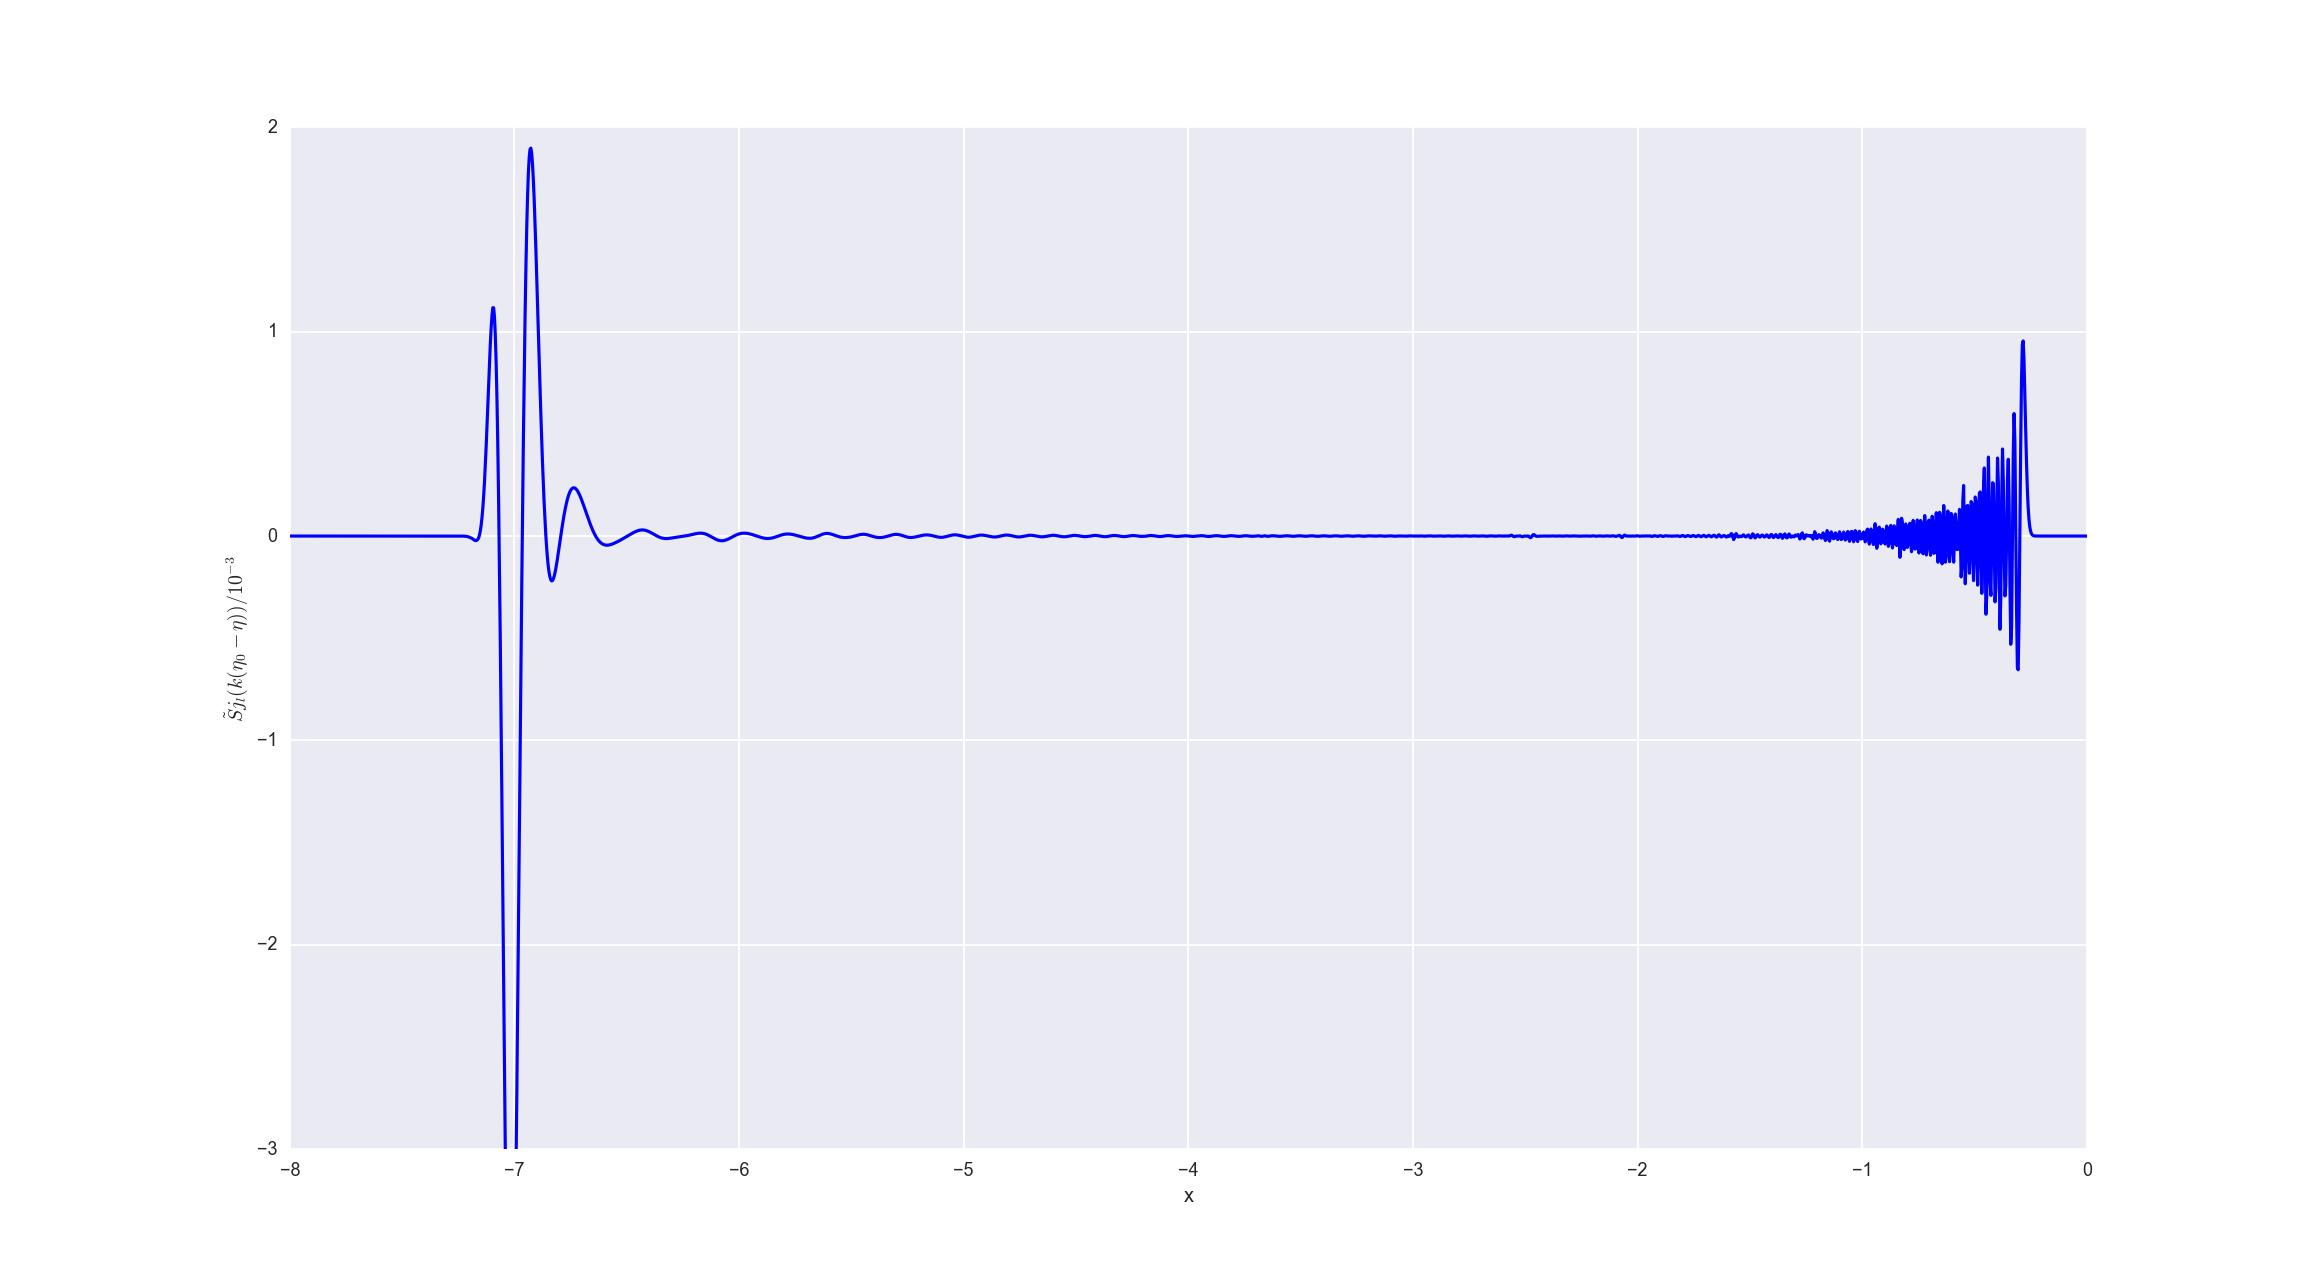
\includegraphics[scale=0.25]{sjl.png}
\caption{This shows the source function multiplied with the spherical Bessel function for $l=100$ and $k = 340\cdot H_0/c$. The plot is more or less the same as in Callin \cite{Callin} except from some spikes at $x\approx -0.5$.}\label{fig:sjl}
\end{figure}

\begin{figure*}[!htbp]
\centering
\begin{tabular}{@{}ccc@{}}
\subfloat[The figure shows a completly unscaled transfer function $\Theta_l(k)$.\label{fig:theta}]{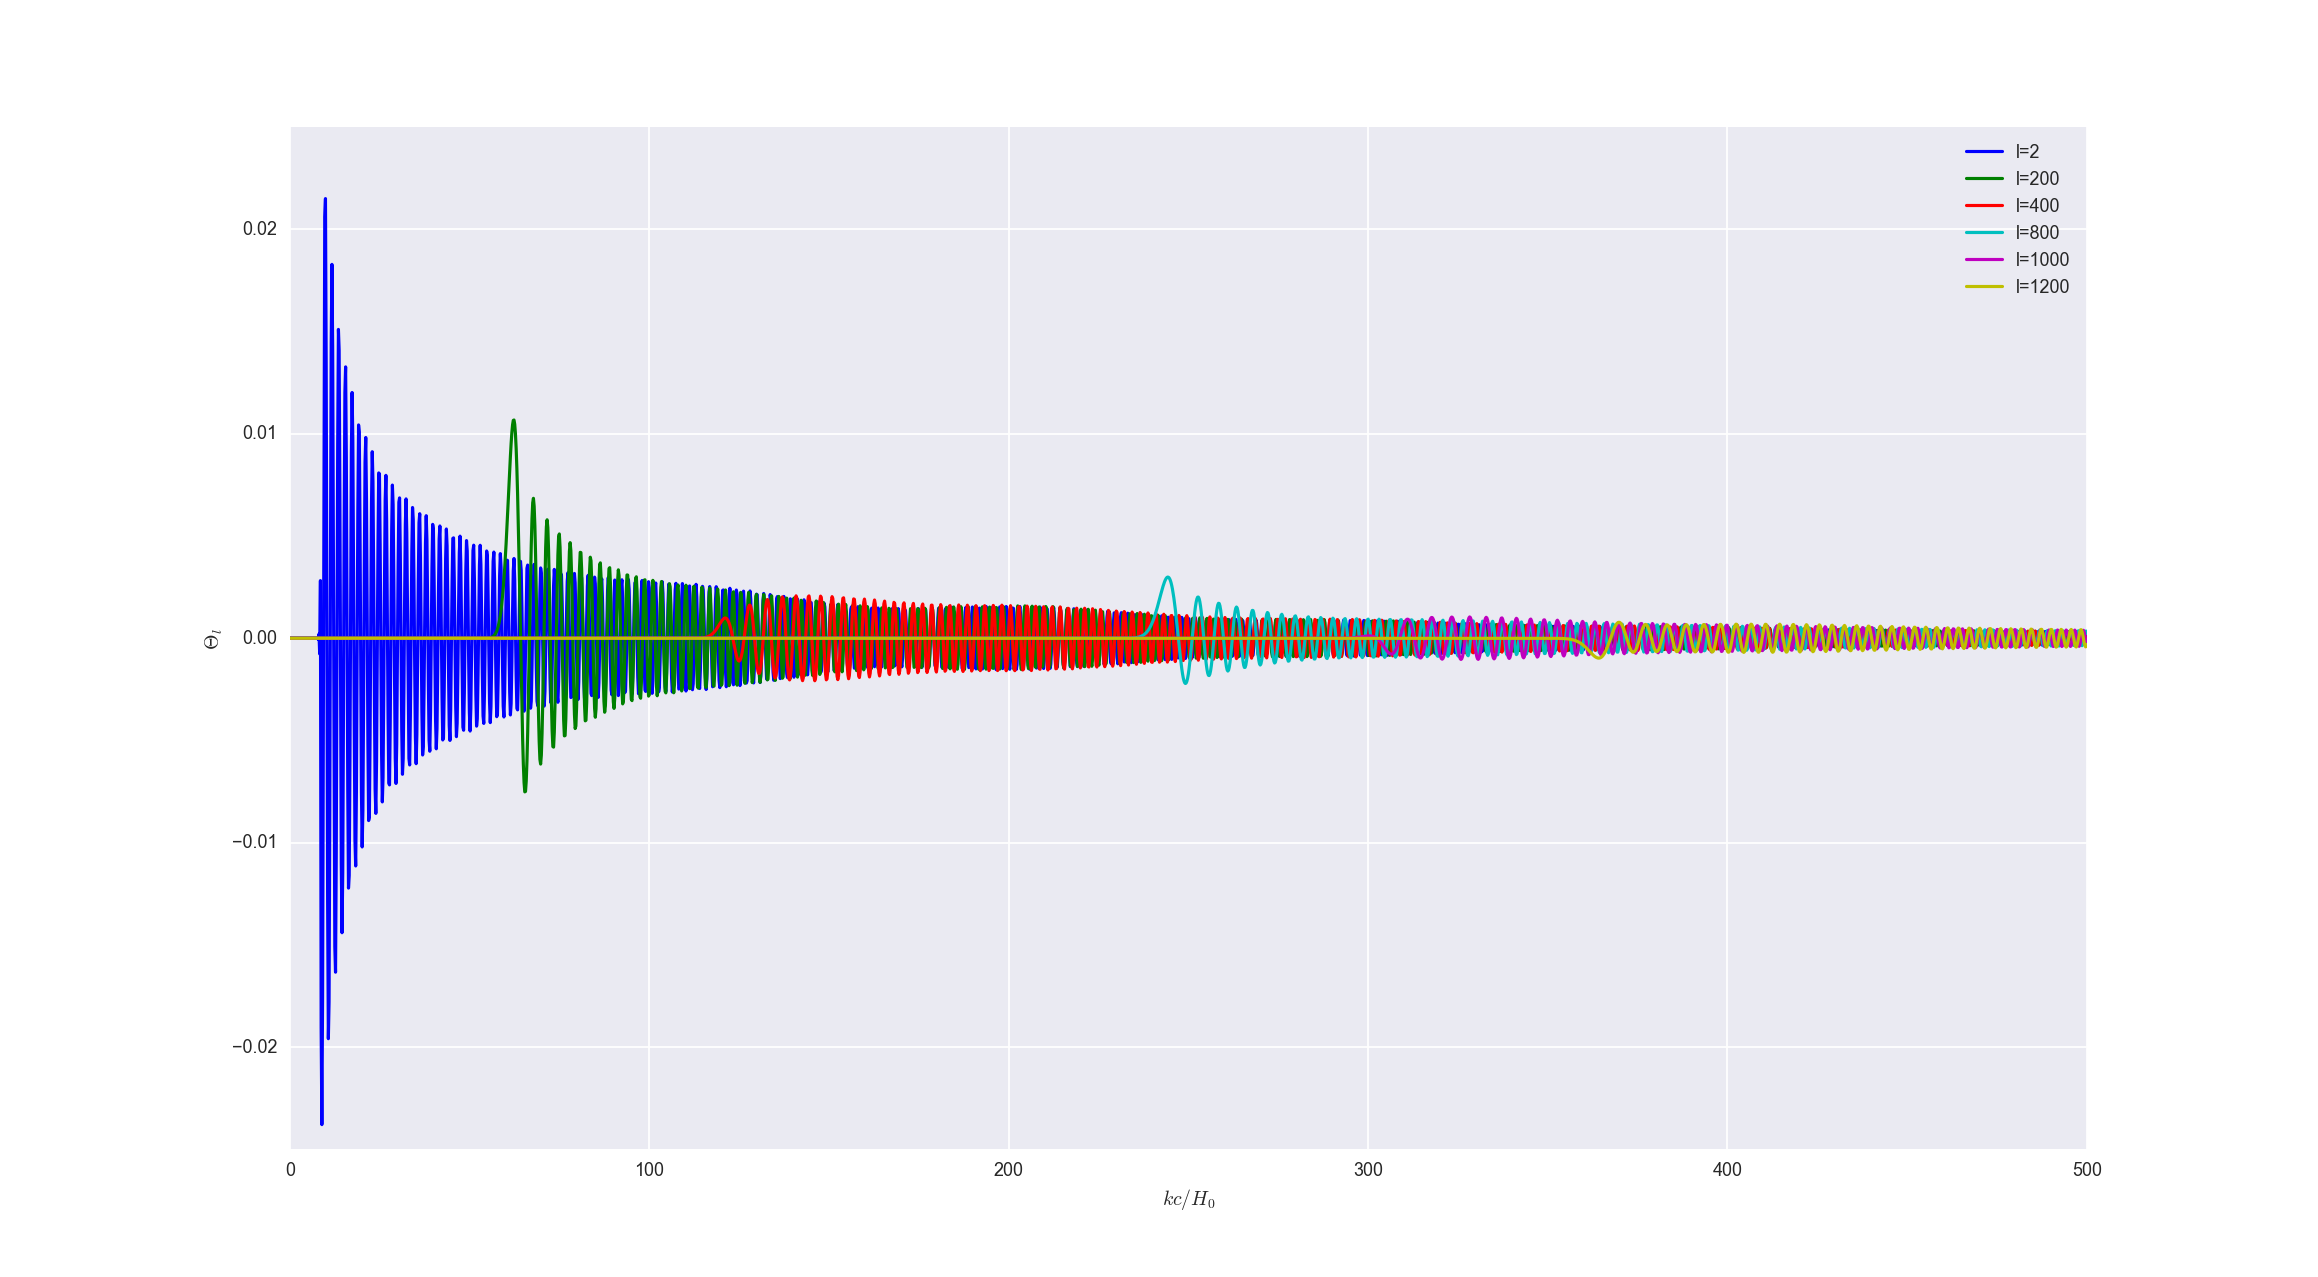
\includegraphics[width=0.5\textwidth]{theta_l.png}} & 
\subfloat[Plot showing $\Theta_l^2(k)/k$. The plots are scaled with $l(l+1)H_0/c$ to make the functions for the different $l$s more similar.\label{fig:theta_sq_k}]{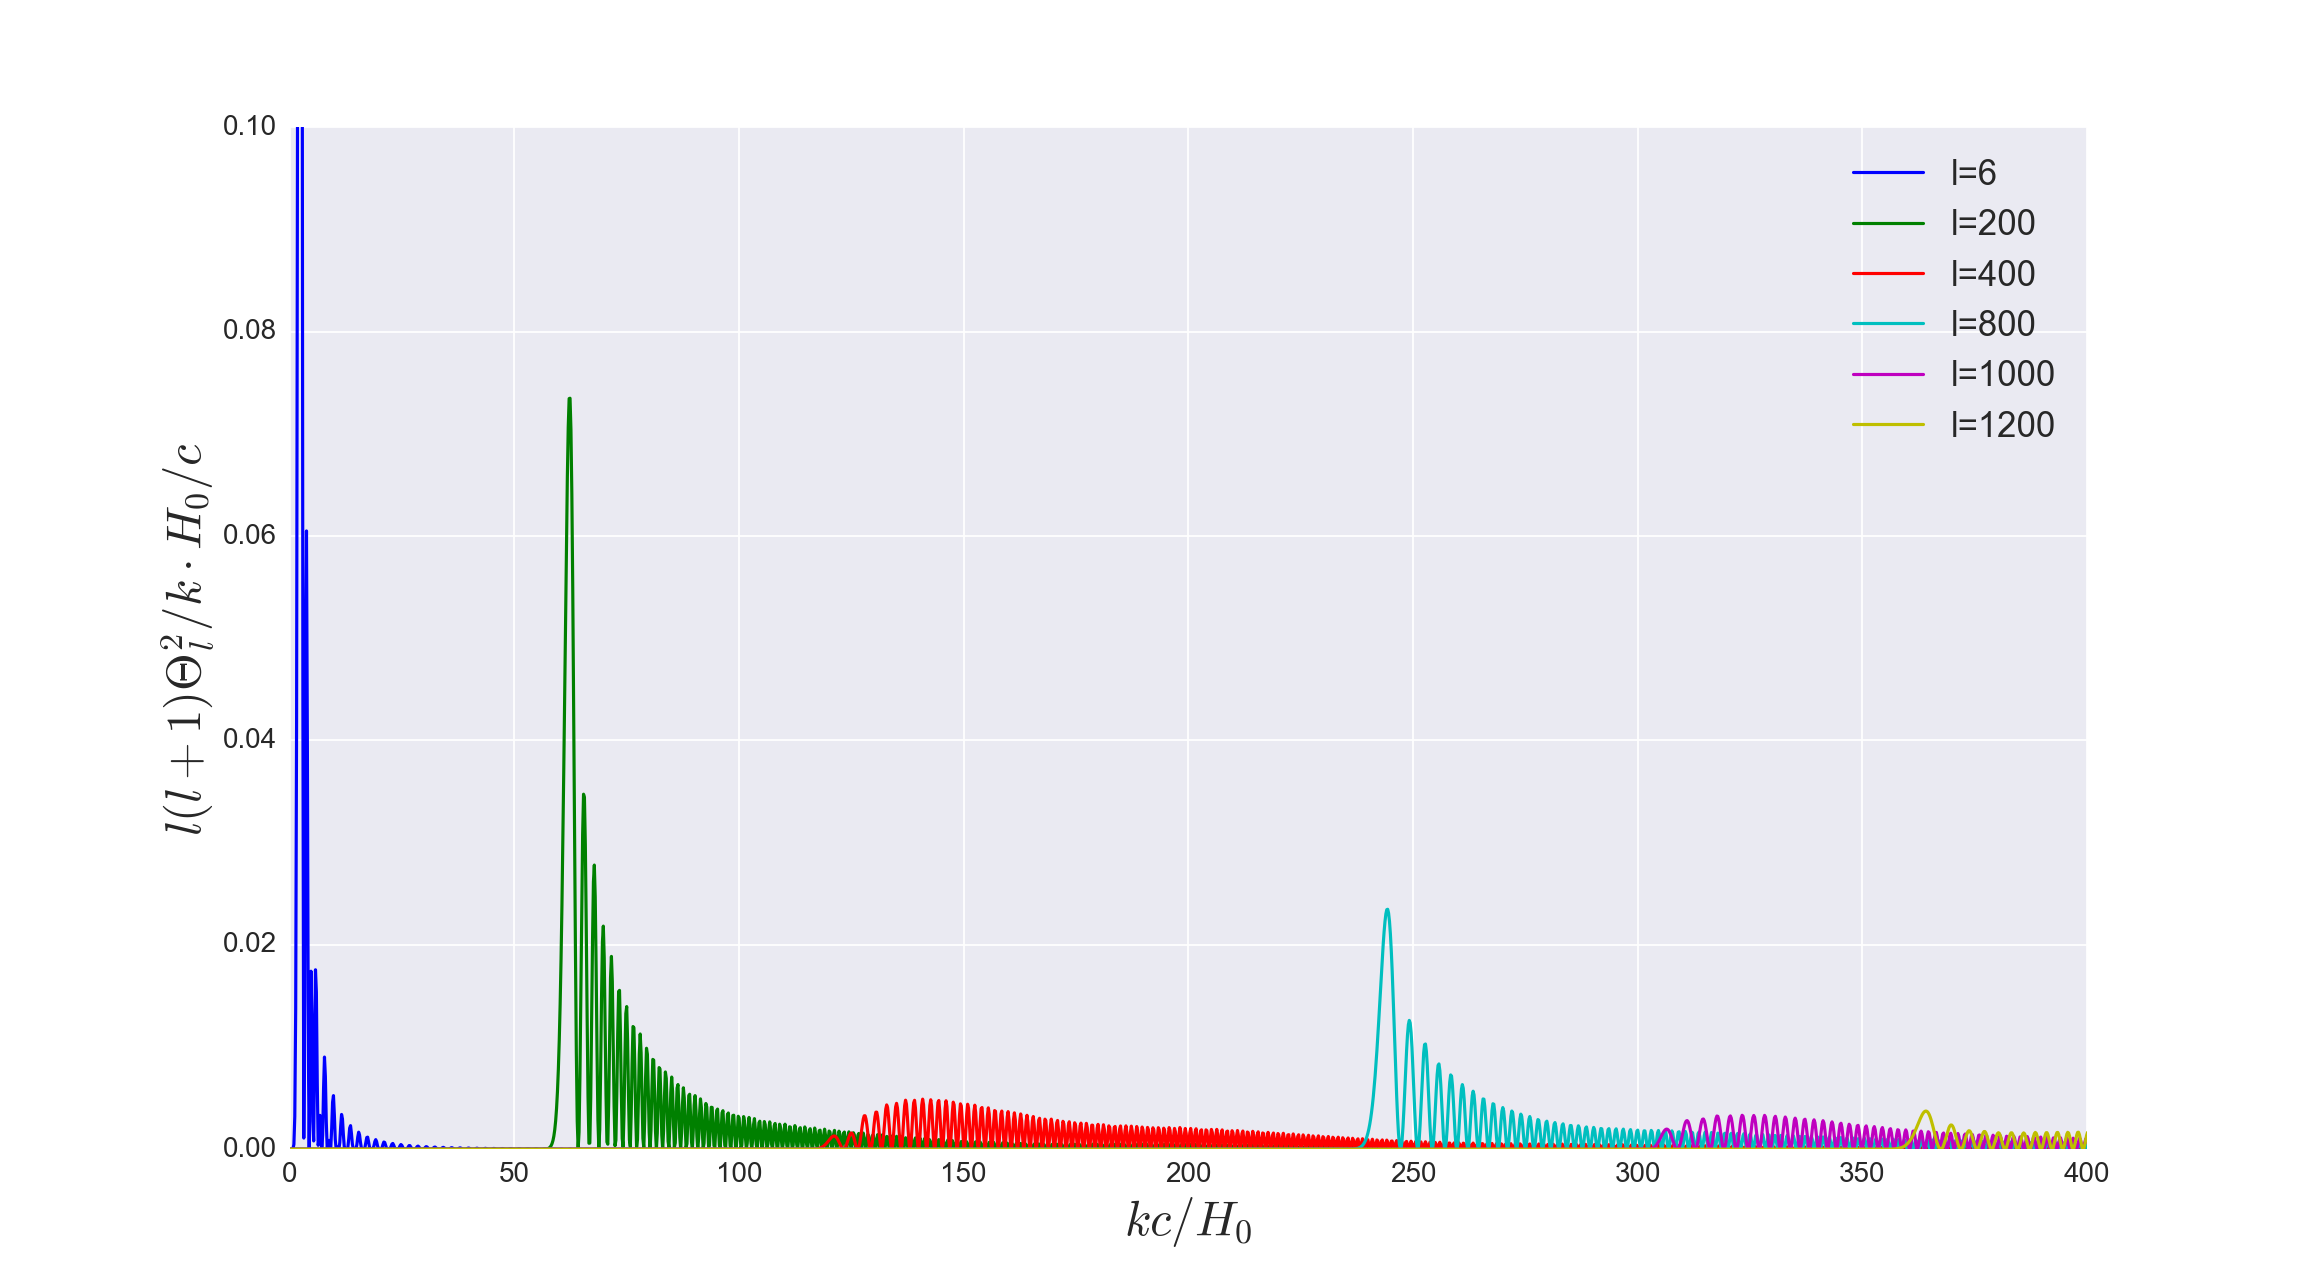
\includegraphics[width=0.5\textwidth]{theta_sq_k.png}} 
\end{tabular}
\caption[]{Plots showing the transfer function $\Theta_l(k)$ for a selection of $l$s.}
\label{fig:thetas}
\end{figure*}

Looking at figure \ref{fig:sjl} we see $\tilde{S}j_l(k(\eta_0 - \eta))$. This is plotted as a sanity check to compare with figure 3 in Callin \cite{callin}. The plot is for $l = 100$ and the closes we can get to $k = 340\cdot H_0/c$.  This is more or less the same plot as Callin got, meaning that we are on the right track. If we look at the transfer function $\Theta_l(k)$ in figure \ref{fig:thetas} we see that the transfer function on all scales are oscillation as damped harmonic oscillators. 

In fig. \ref{fig:theta_sq_k} we see that generally the scaled $l(l+1)\cdot \Theta_l^2/k$ seems to decrease for larger $l$, and have shapes similar to the damped harmonic oscillator of $\Theta_l$.

\subsection{Power Spectrum $C_l$}
The first power spectrum calculated is with the parameters found in the \textit{Default} row of table \ref{tab:parameters}. 

\begin{table}[!htb]
\centering
\begin{tabular}{l c c c c c}
& $\Omega_b$ & $\Omega_m$ & $\Omega_r$ & $n_s$ & $h$ \\
\hline 
Default & $0.046$ & $0.224$ & $8.3\cdot 10^{-5}$ & $0.967$ & $0.7$ \\
Best Fit & $0.065$ & $0.20$ & $8.3\cdot 10^{-5}$ & $0.80$ & $0.7$ \\

\end{tabular}
\caption{Parameters used for the default power spectrum and the best fit.}\label{tab:parameters}
\end{table}

\begin{figure}[!htp]
\centering
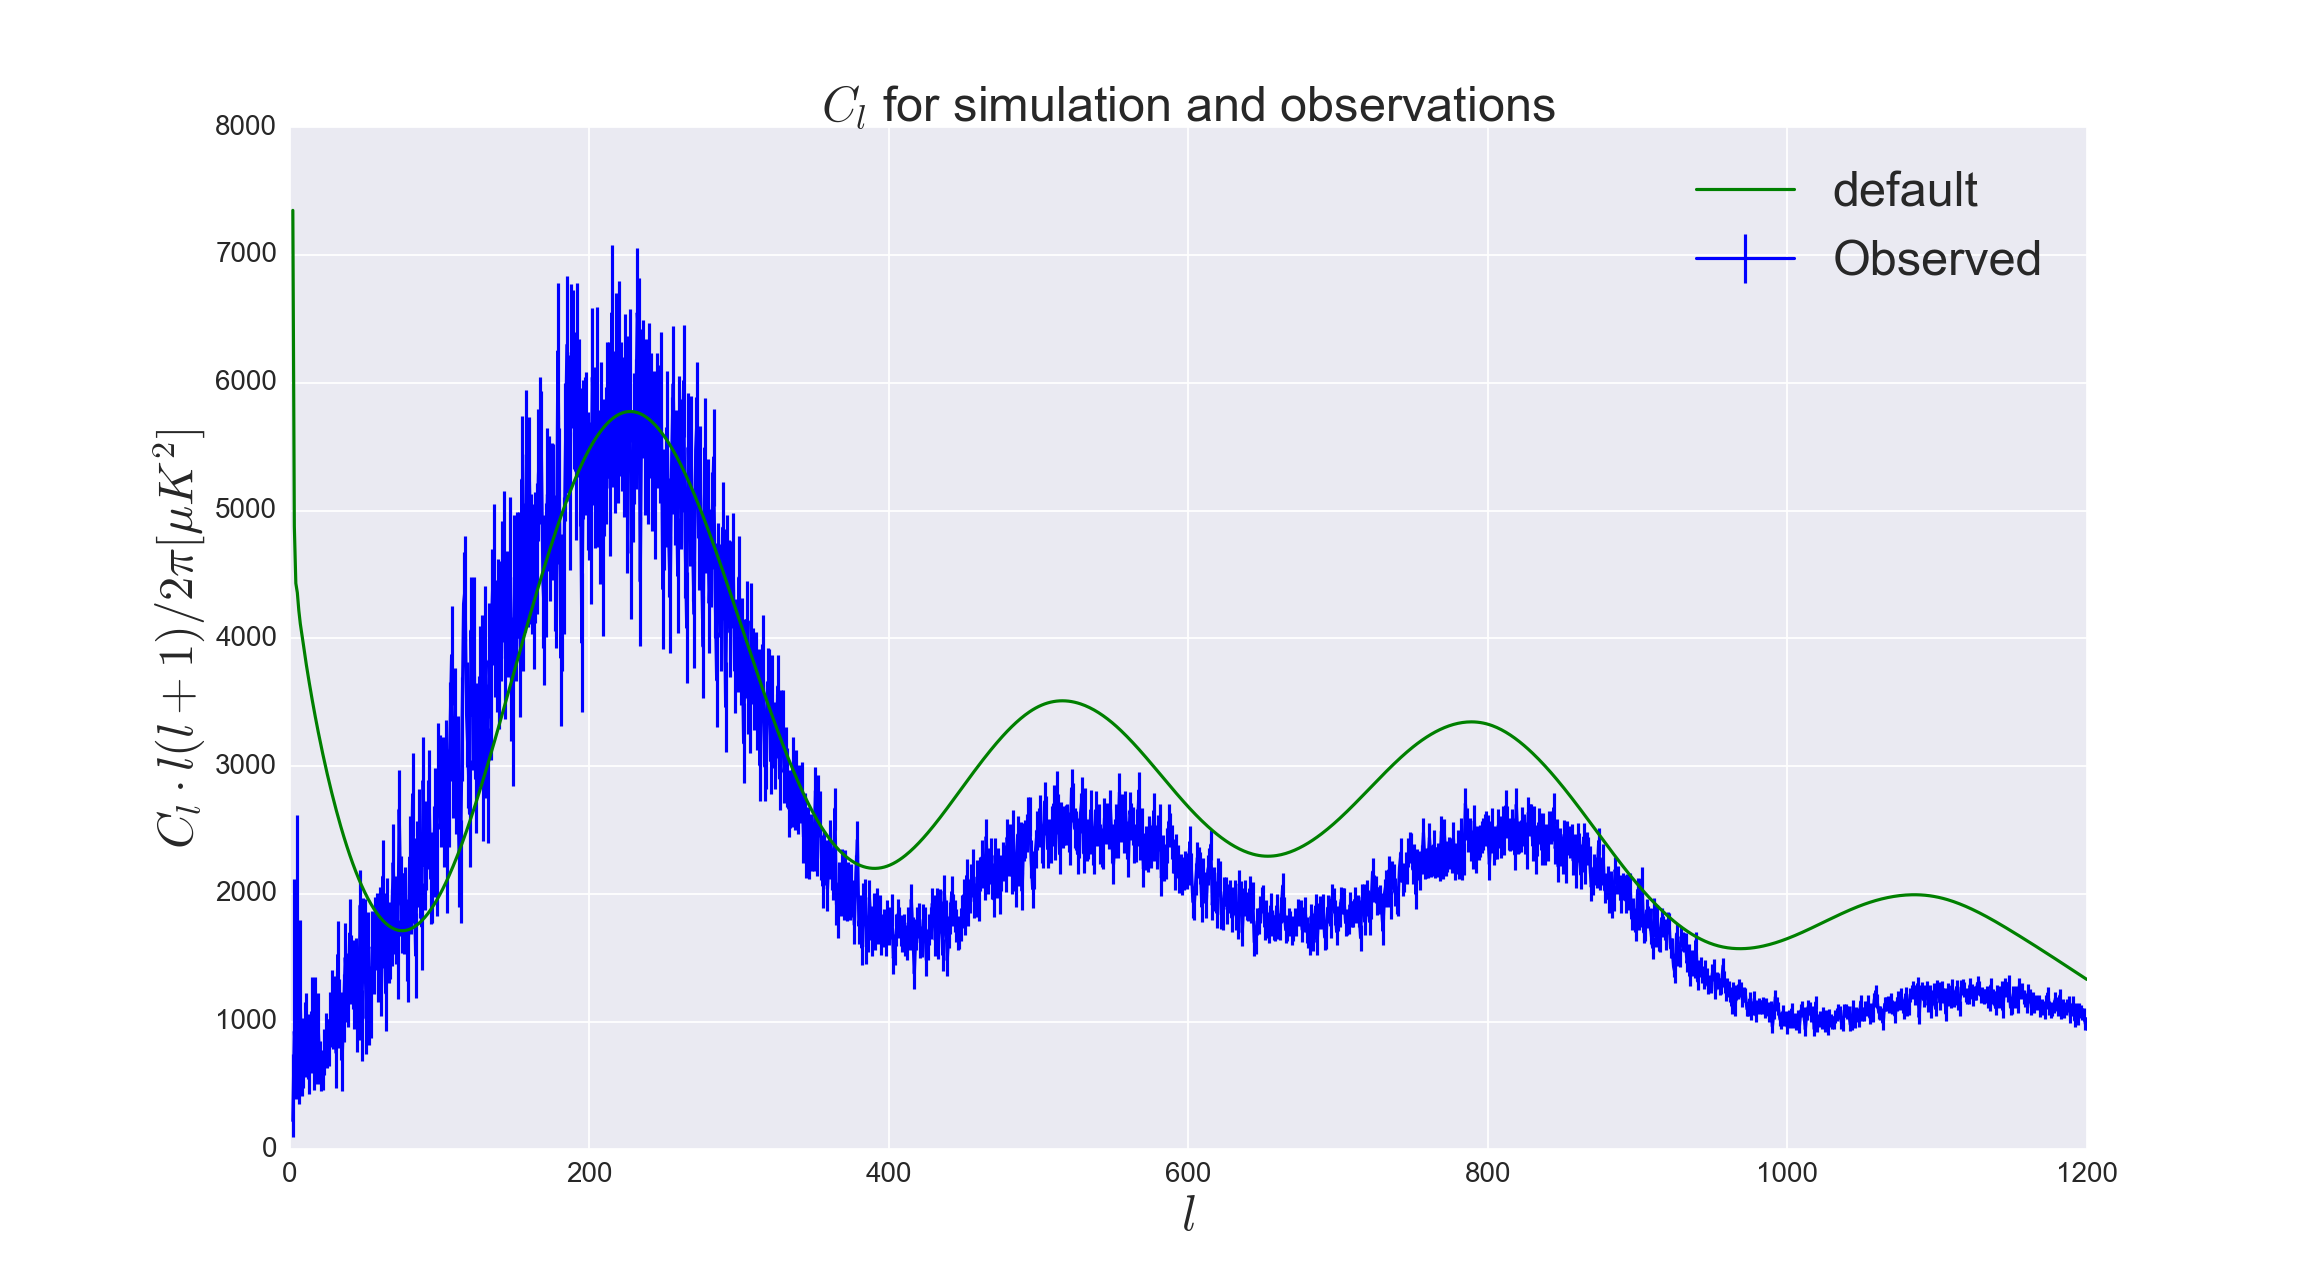
\includegraphics[scale=0.25]{Cl.png}
\caption{The power spectrum $C_l l(l+1)/2\pi$ in $\mu K^2$. We see that thoug it has the same shape as the Planck data, the values after the acoustic peak is a bit to low. We can also see that for low $l$s the power spectrum as a way to large value.}\label{fig:Cl_default}
\end{figure}

The resulting power spectrum can be seen in figure \ref{fig:Cl_default}. Since the top of the first acoustic peak in both the simulated data and in the Planck data is normalized to be at $5775 \mu K^2$, they will always agree here. After the peak there is disagreement between the simulated result and the observations, with the simulated $C_l$ having a higher value. Before the peak there is agreement above $l \approx 90$; below this the simulated data shoots upwards, and at $l \approx 2$ there is only mess... This problem is not removed by adjusting the parameters -- have not test by changing $\Omega_k$ and $\Omega_{\Lambda}$, even though they have alot to say for small $l$s --, and will in some instances make it worse. There is most likely some expression somewhere in the code that is wrong, but I've yet to find it.

\begin{figure*}[!htbp]
\centering
\begin{tabular}{@{}ccc@{}}
\subfloat[$C_l$ when the spectral index $n_s$ is changed. We see that with a lower $n_s$, $C_l$ decreases. The increase for smaller $l$s is due to the normalization at the peak of the acoustic peak. \label{fig:Cl_n}]{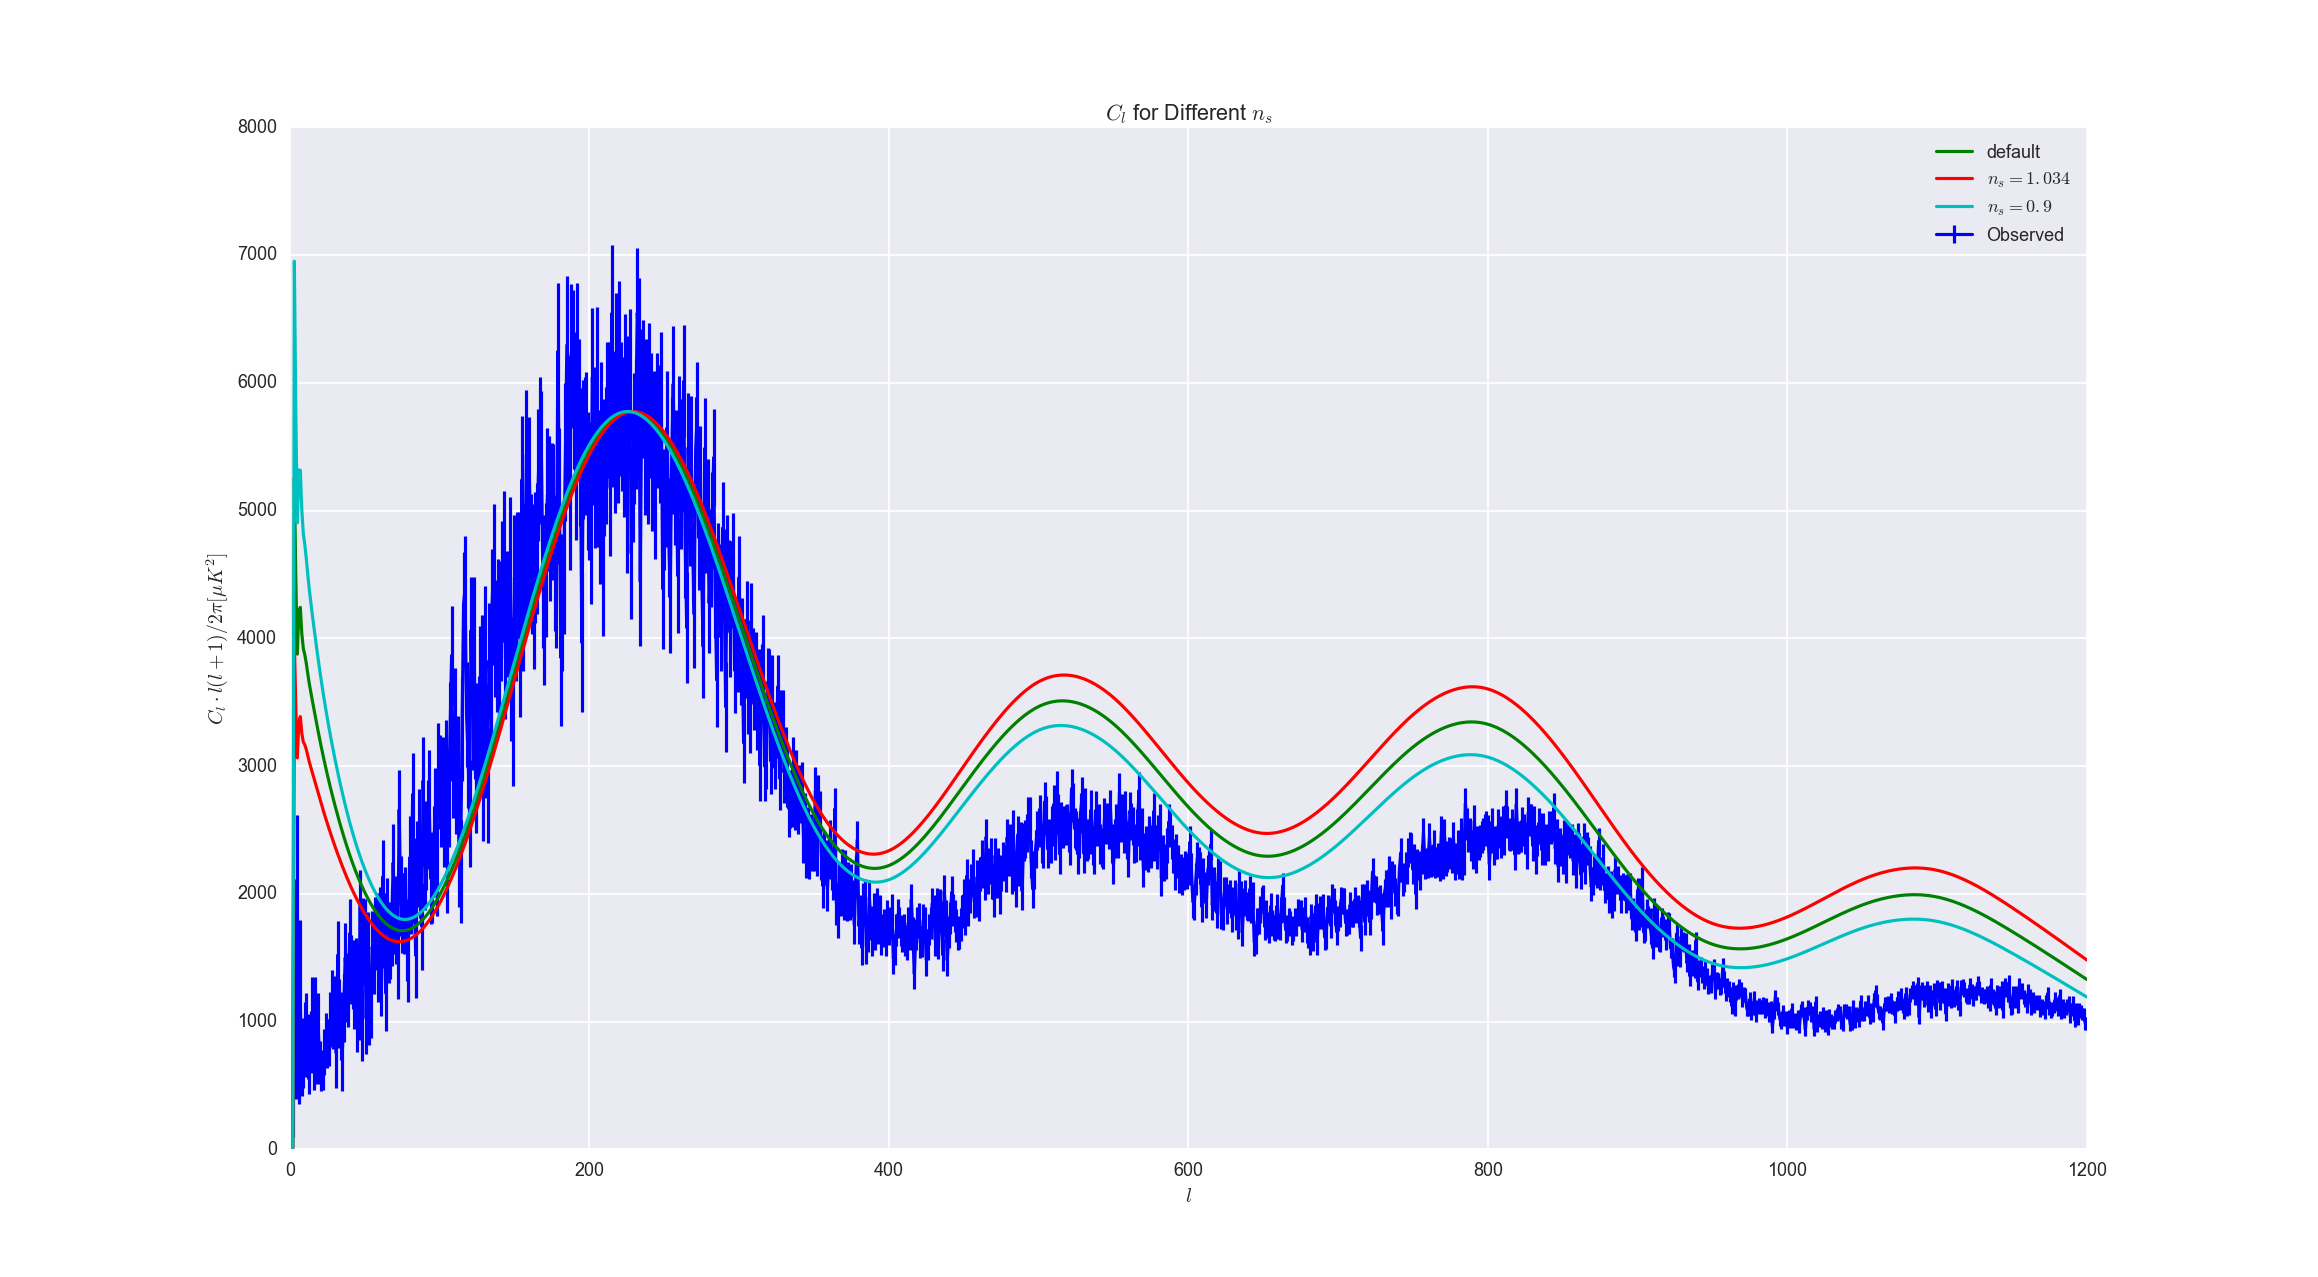
\includegraphics[width=0.5\textwidth]{Cl_n.png}} & 
\subfloat[$C_l$ when the dimensionless Hubble parameter $h$ is changed. We see that there is not much difference when the change in the range that would expect to see. \label{fig:Cl_h}]{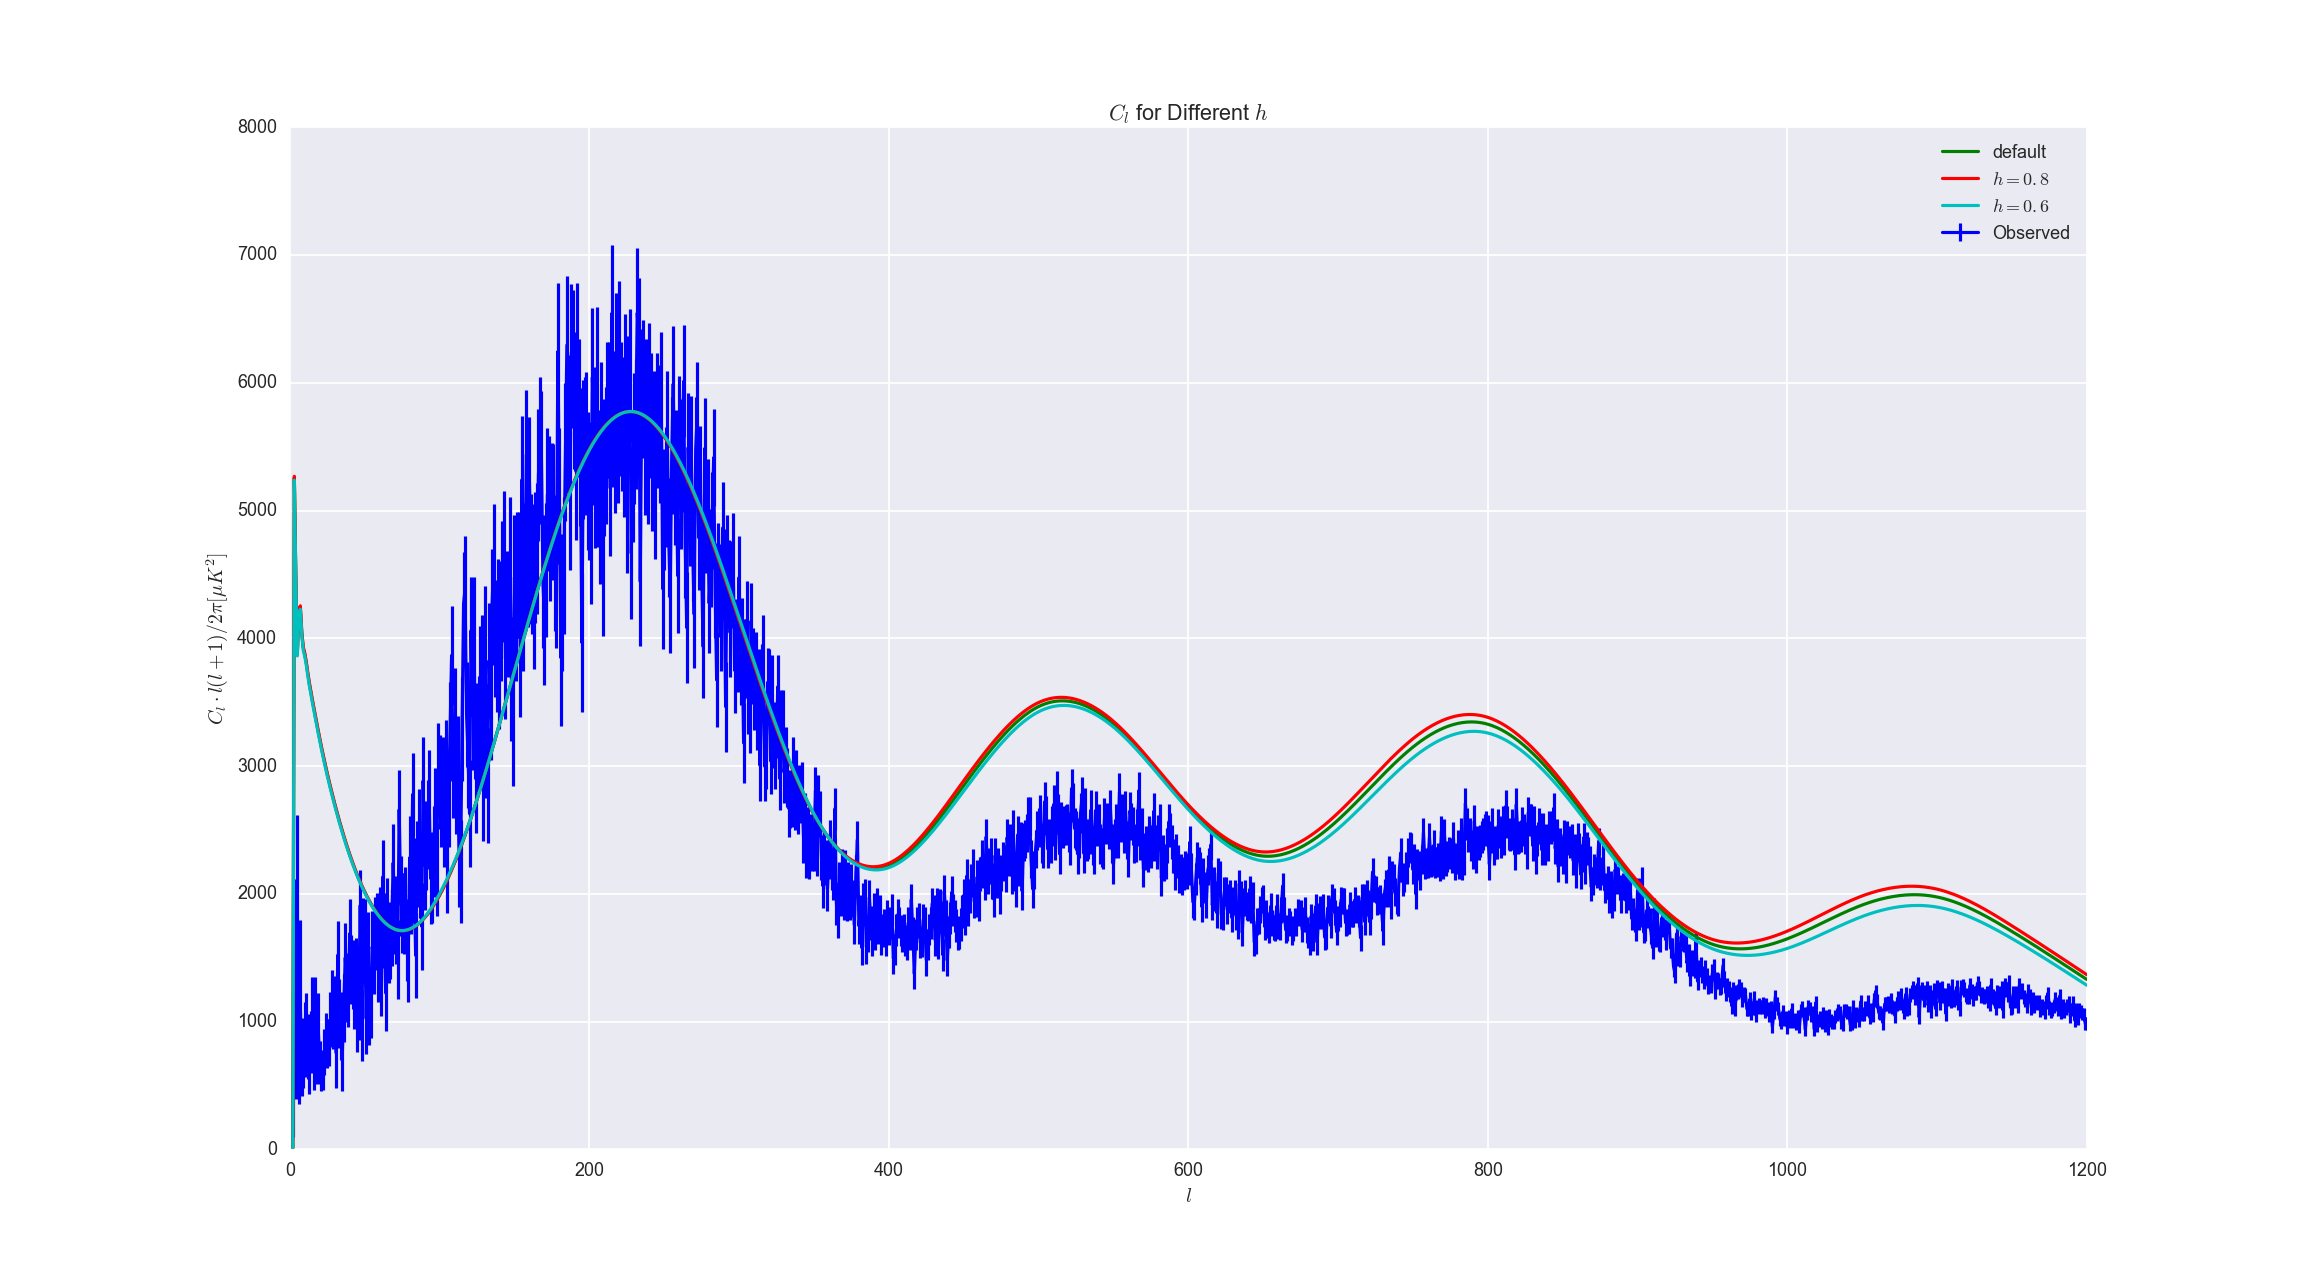
\includegraphics[width=0.5\textwidth]{Cl_h.png}} \\
\subfloat[$C_l$ when the density parameter of baryons $\Omega_b$ is changed. We see that for when $\Omega_b$ is higher, there are more baryons, meaning they are able to compress more, and decompress less, meaning that the second compression peak now are larger than the first decompression peak. The opposite is true when decreases $\Omega_b$.\label{fig:Cl_b}]{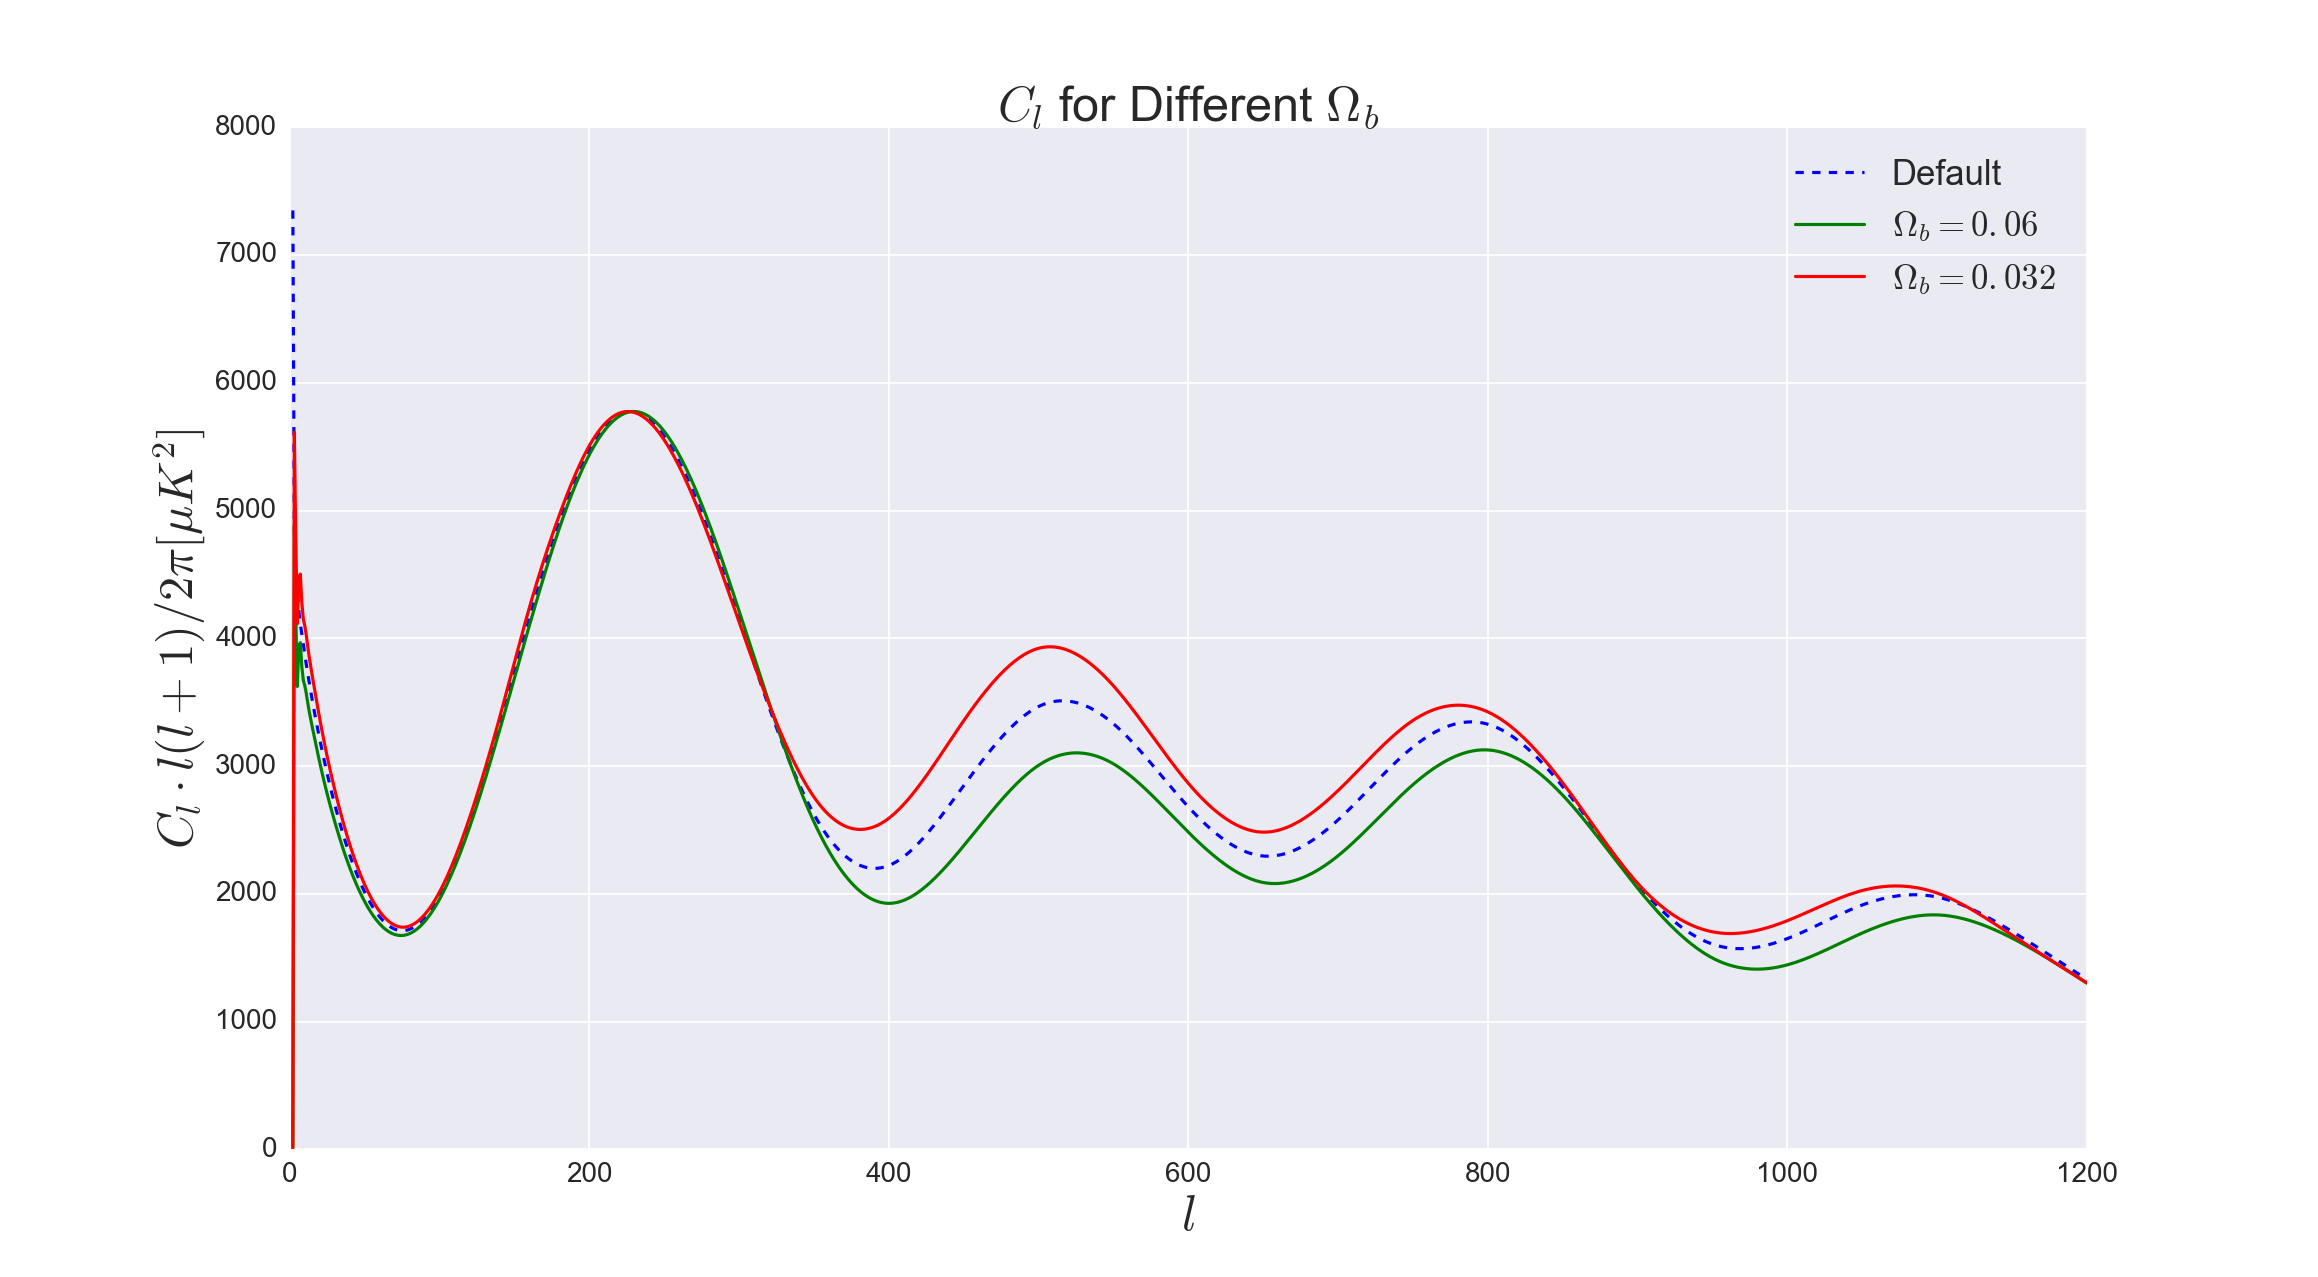
\includegraphics[width=0.5\textwidth]{Cl_b.png}} & 
\subfloat[$C_l$ when the density parameter of cold dark matter $\Omega_m$ is changed. With a higher $\Omega_m$, the main effect here is that since dark matter is more prevalent, recombination will happen later, moving the first compression peak towards smaller $l$s. The second effect is to lower all peaks, this is not seen here, since we normalize the first compression peak. This makes it look like higher $\Omega_m$ increases the peaks. The opposite is true when decreases $\Omega_m$.\label{fig:Cl_m}]{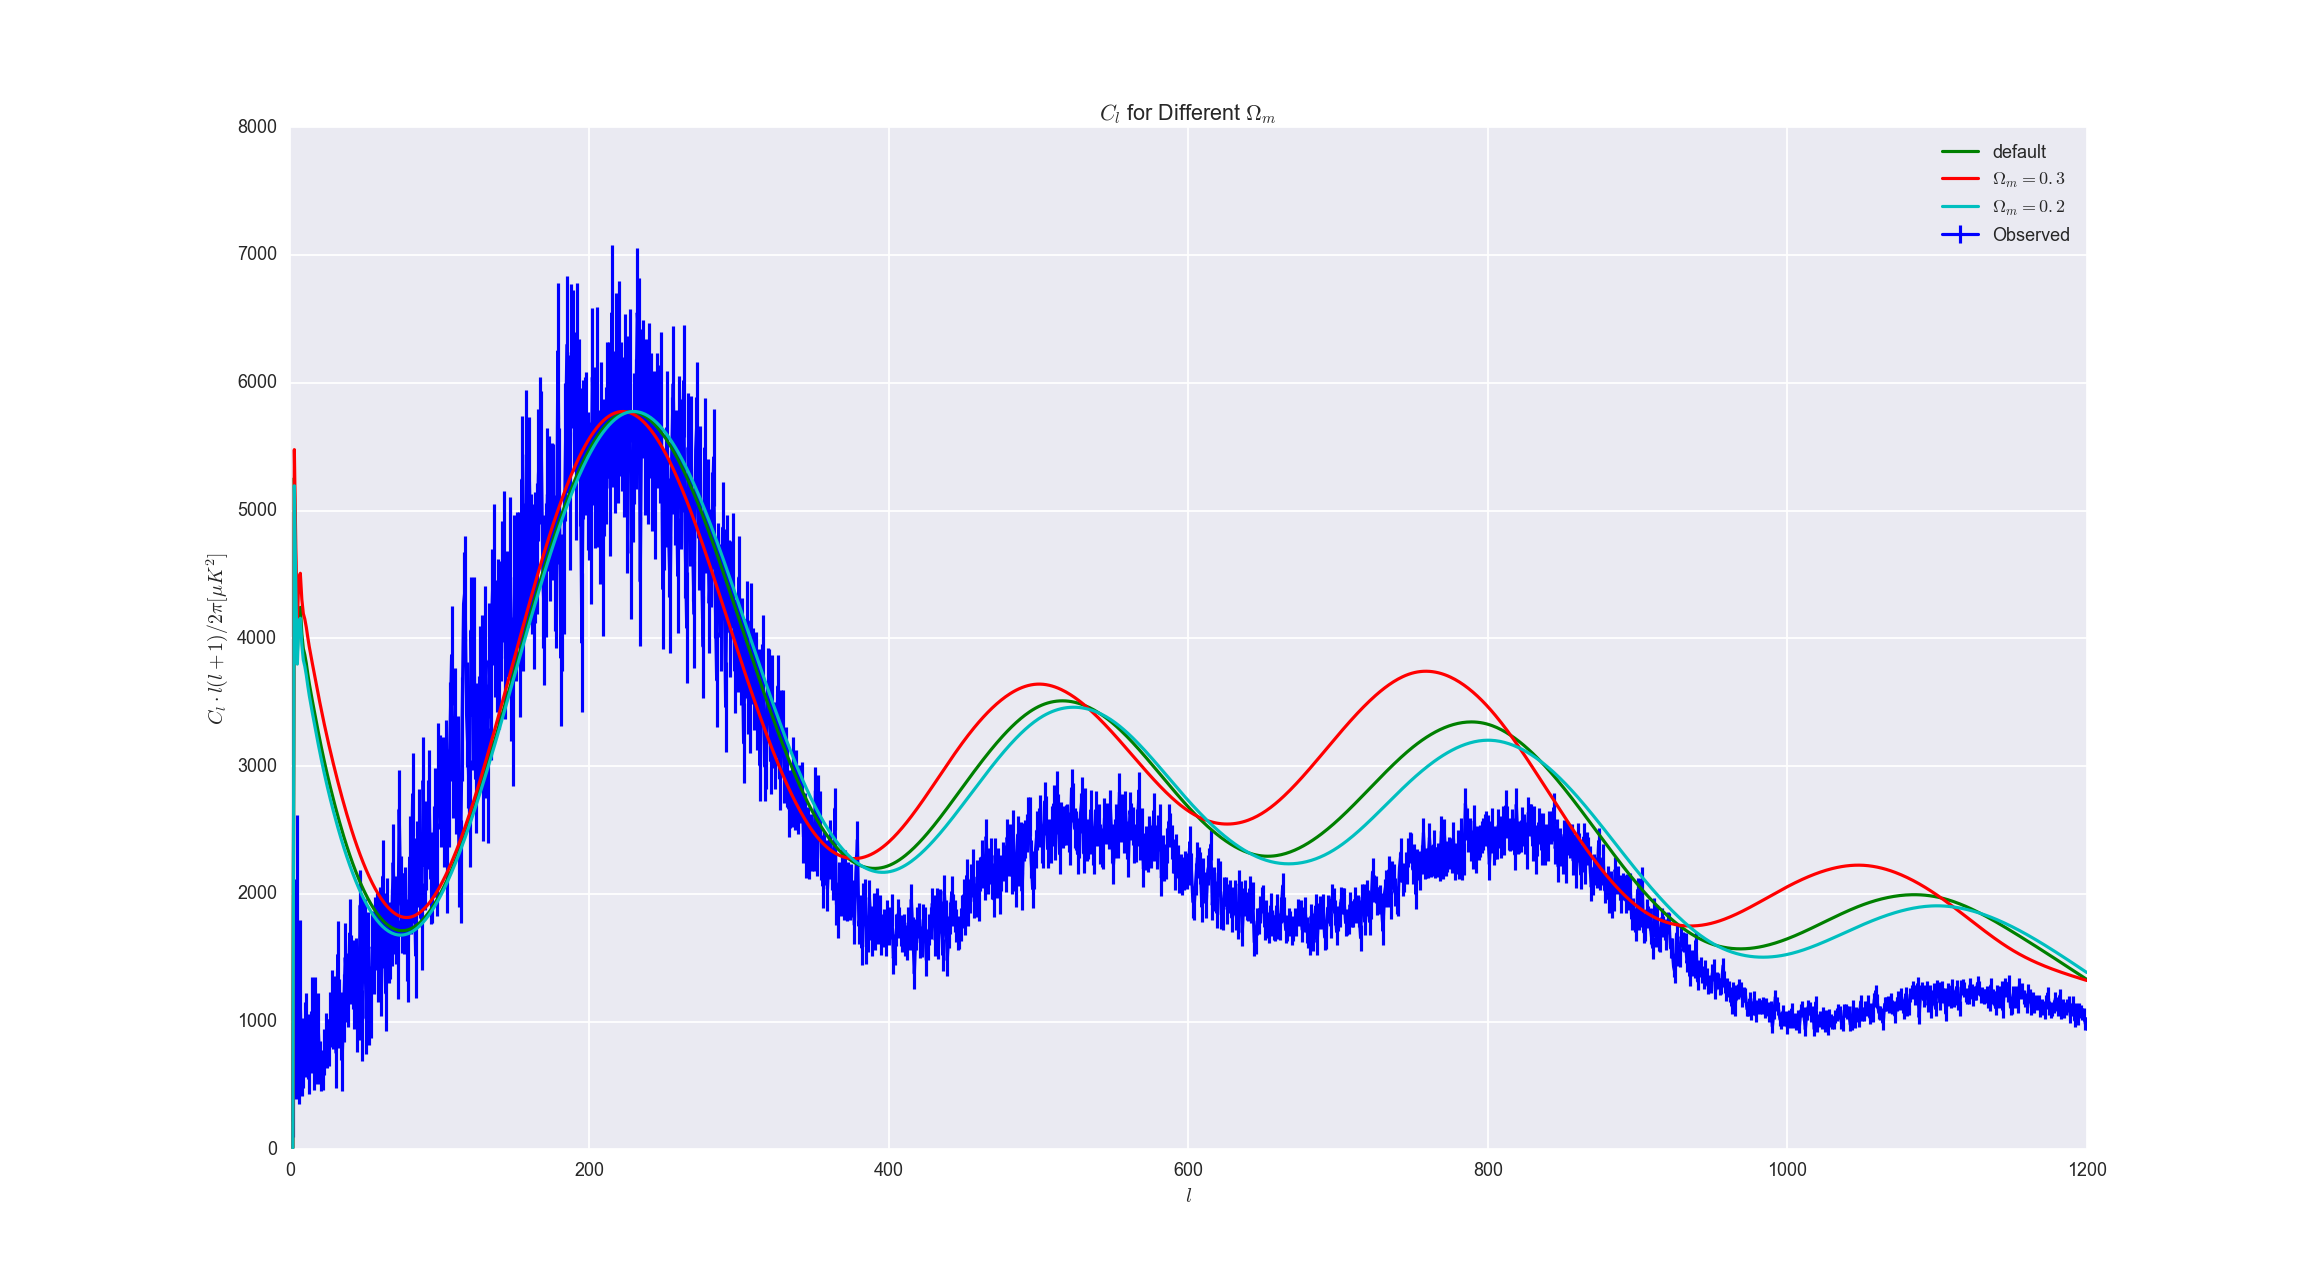
\includegraphics[width=0.5\textwidth]{Cl_m.png}} \\
\subfloat[$C_l$ when the density parameter of radiation $\Omega_r$ is changed. With a higher $\Omega_r$ recombination seems to happen earlier, this pushing the first compression peak to higher $l$s. It also streches the distance between the peaks. Since we now have more radiation the pressure in the compressed baryon-photon fluid is higher, and thus the first decompression peak is higher than the second compression peak. The opposite is true when decreases $\Omega_r$.\label{fig:Cl_r}]{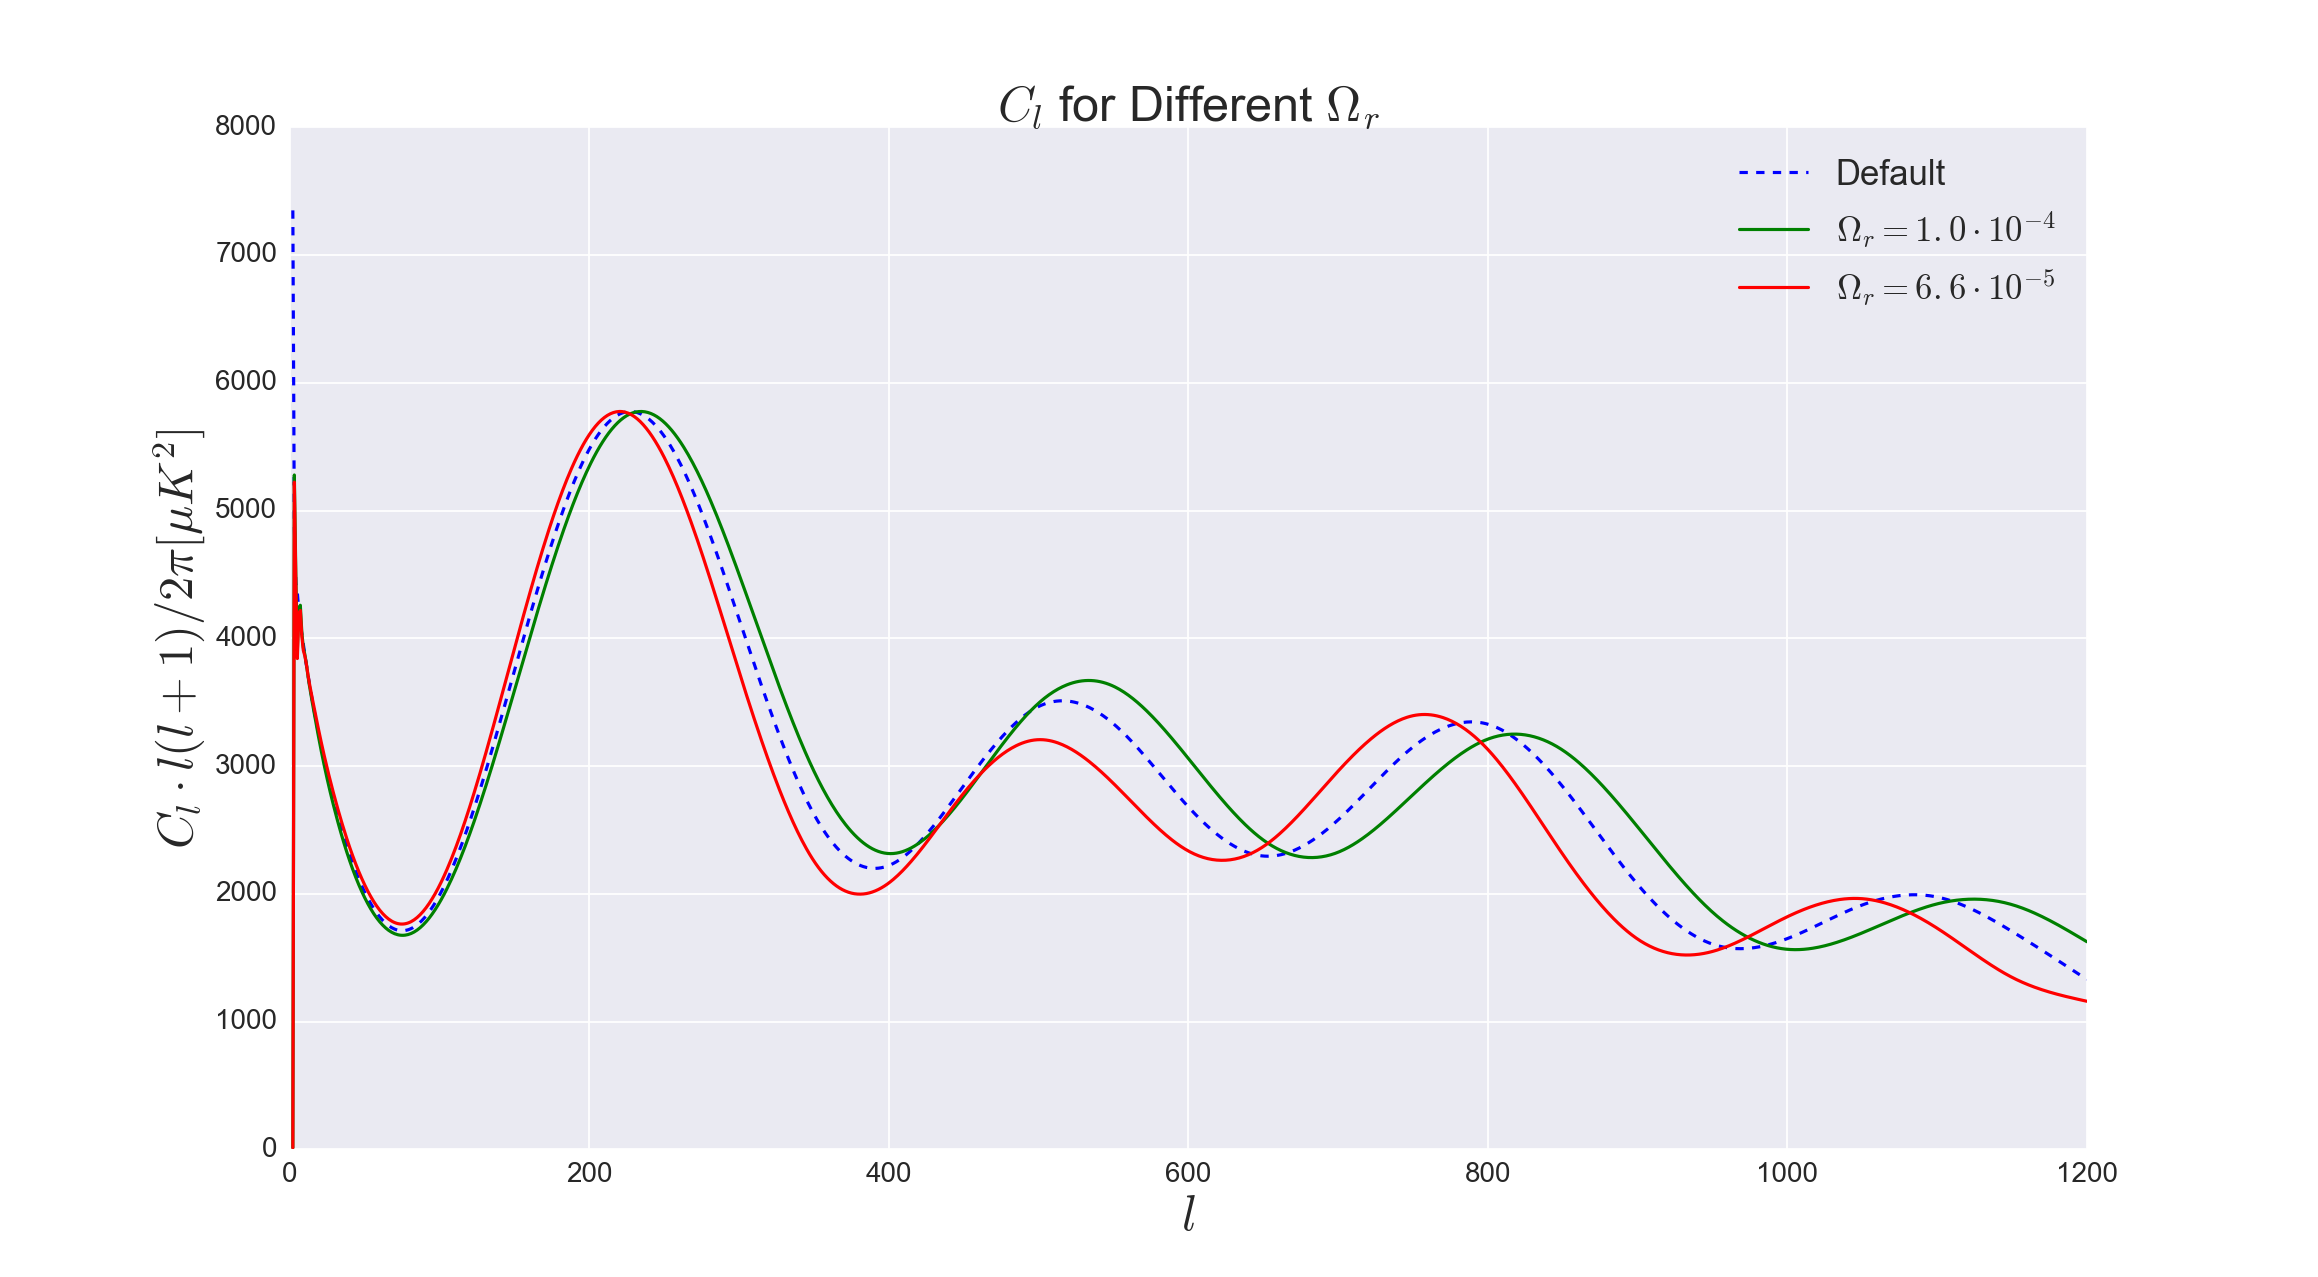
\includegraphics[width=0.5\textwidth]{Cl_r.png}} 
\end{tabular}
\caption[]{Plots showing the differences in the the power spectrum $C_l$ when changing the five parameters one by one.}
\label{fig:Cl_changed}
\end{figure*}


Figure \ref{fig:Cl_changed} we see that happens when each of the parameters are changed one by one. Below I describe what happens when the parameters are increased, but the opposite should happen if they are decreased (as the plots show).

\subsubsection{$n_s$}
The result is showed in fig. \ref{fig:Cl_n}. Since we have the primordial power spectrum found in eq. \ref{eq:P} there is a strong dependence on $n_s$. If we have a non-unity $n_s$ the primordial power spectrum will depend on scale. With a $n_s<1$ the primordial power spectrum decreases on smaller scales, and the same would be true for $C_l$. This is what we see from fig. \ref{fig:Cl_n}. But in the figure we see that $C_l$ increases if $l< 220$. This is because we have renormalized so that all the first acoustic peaks have the same hight.

\subsubsection{$h$}
Since many of the equation used in our calculation is dependent on $H_0$ and thus the dimensionless Hubble parameter $h$, we would expect to see differences when changing it. But from fig. \ref{fig:Cl_h} we see that the changes are very small.

\subsubsection{$\Omega_b$}
$\Omega_b$, fig. \ref{fig:Cl_b}, determines the amount of baryons in the Universe. With more baryon the gravitation wells the baryon-photon fluid collapses into are deeper, and the compressions are larger and decompressions smaller. This is why we see that the ratio between the compression/decompression peaks are larger. The first compression peak should also higher, and the ratio between this and the rest of the peaks should be larger, but due to the normalization it stays the same, while the later peaks decrease. More baryons also changes the sound speed(and thus the sound horizon), and the first peak shifts to higher $l$s. This effect can be seen, but is very small.

\subsubsection{$\Omega_m$}
$\Omega_m$, fig. \ref{fig:Cl_m}, determines the amount of cold dark matter in the Universe. A larger amount of dark matter would make a deeper gravitational well, which will dampen the acoustic oscillations, so the peaks decay faster. It would also decrease all peaks, but due to the normalization the first compression peak is always the same hight, while the later peaks decreases. Since dark matter makes up the larger part of matter, an increase in dark matter starts matter domination earlier and thus recombination happens later. As we see in fig. \ref{fig:Cl_m} the first peak is towards lower $l$s thus happening	 later.

\subsubsection{$\Omega_r$}
$\Omega_r$, fig. \ref{fig:Cl_r}, determines the amount of radiation -- relativistic particles -- in the Universe. When the the baryon-photon fluid oscillates it is the radiation which makes the pressure. So with more radiation the compression should be weaker and the decompression stronger. This is what we see in fig. \ref{fig:Cl_r}. We also see that the peaks are farther from each other.

\subsection{The Best Fit Parameters}

So since we have to decrease the later peaks, the easiest parameters to change is $\Omega_b$, $\Omega_m$ and $n_s$. We are going to vary $\Omega_b$, $\Omega_m$ and $n_s$. Figure \ref{fig:Cl_bf} shows the result for four different combinations. I chose the purple as the best fit, but a better fit would be somewhere between the light blue and purple. The parameters for this power spectrum is found in table \ref{tab:parameters}. We see that we have a quite good fit, but there is still problems for smaller $l$s. 

It is possible to use $\Omega_r$ and $h$ and try to make better fit, but was not done due to time restrictions. 


\begin{figure}[!htbp]
\centering
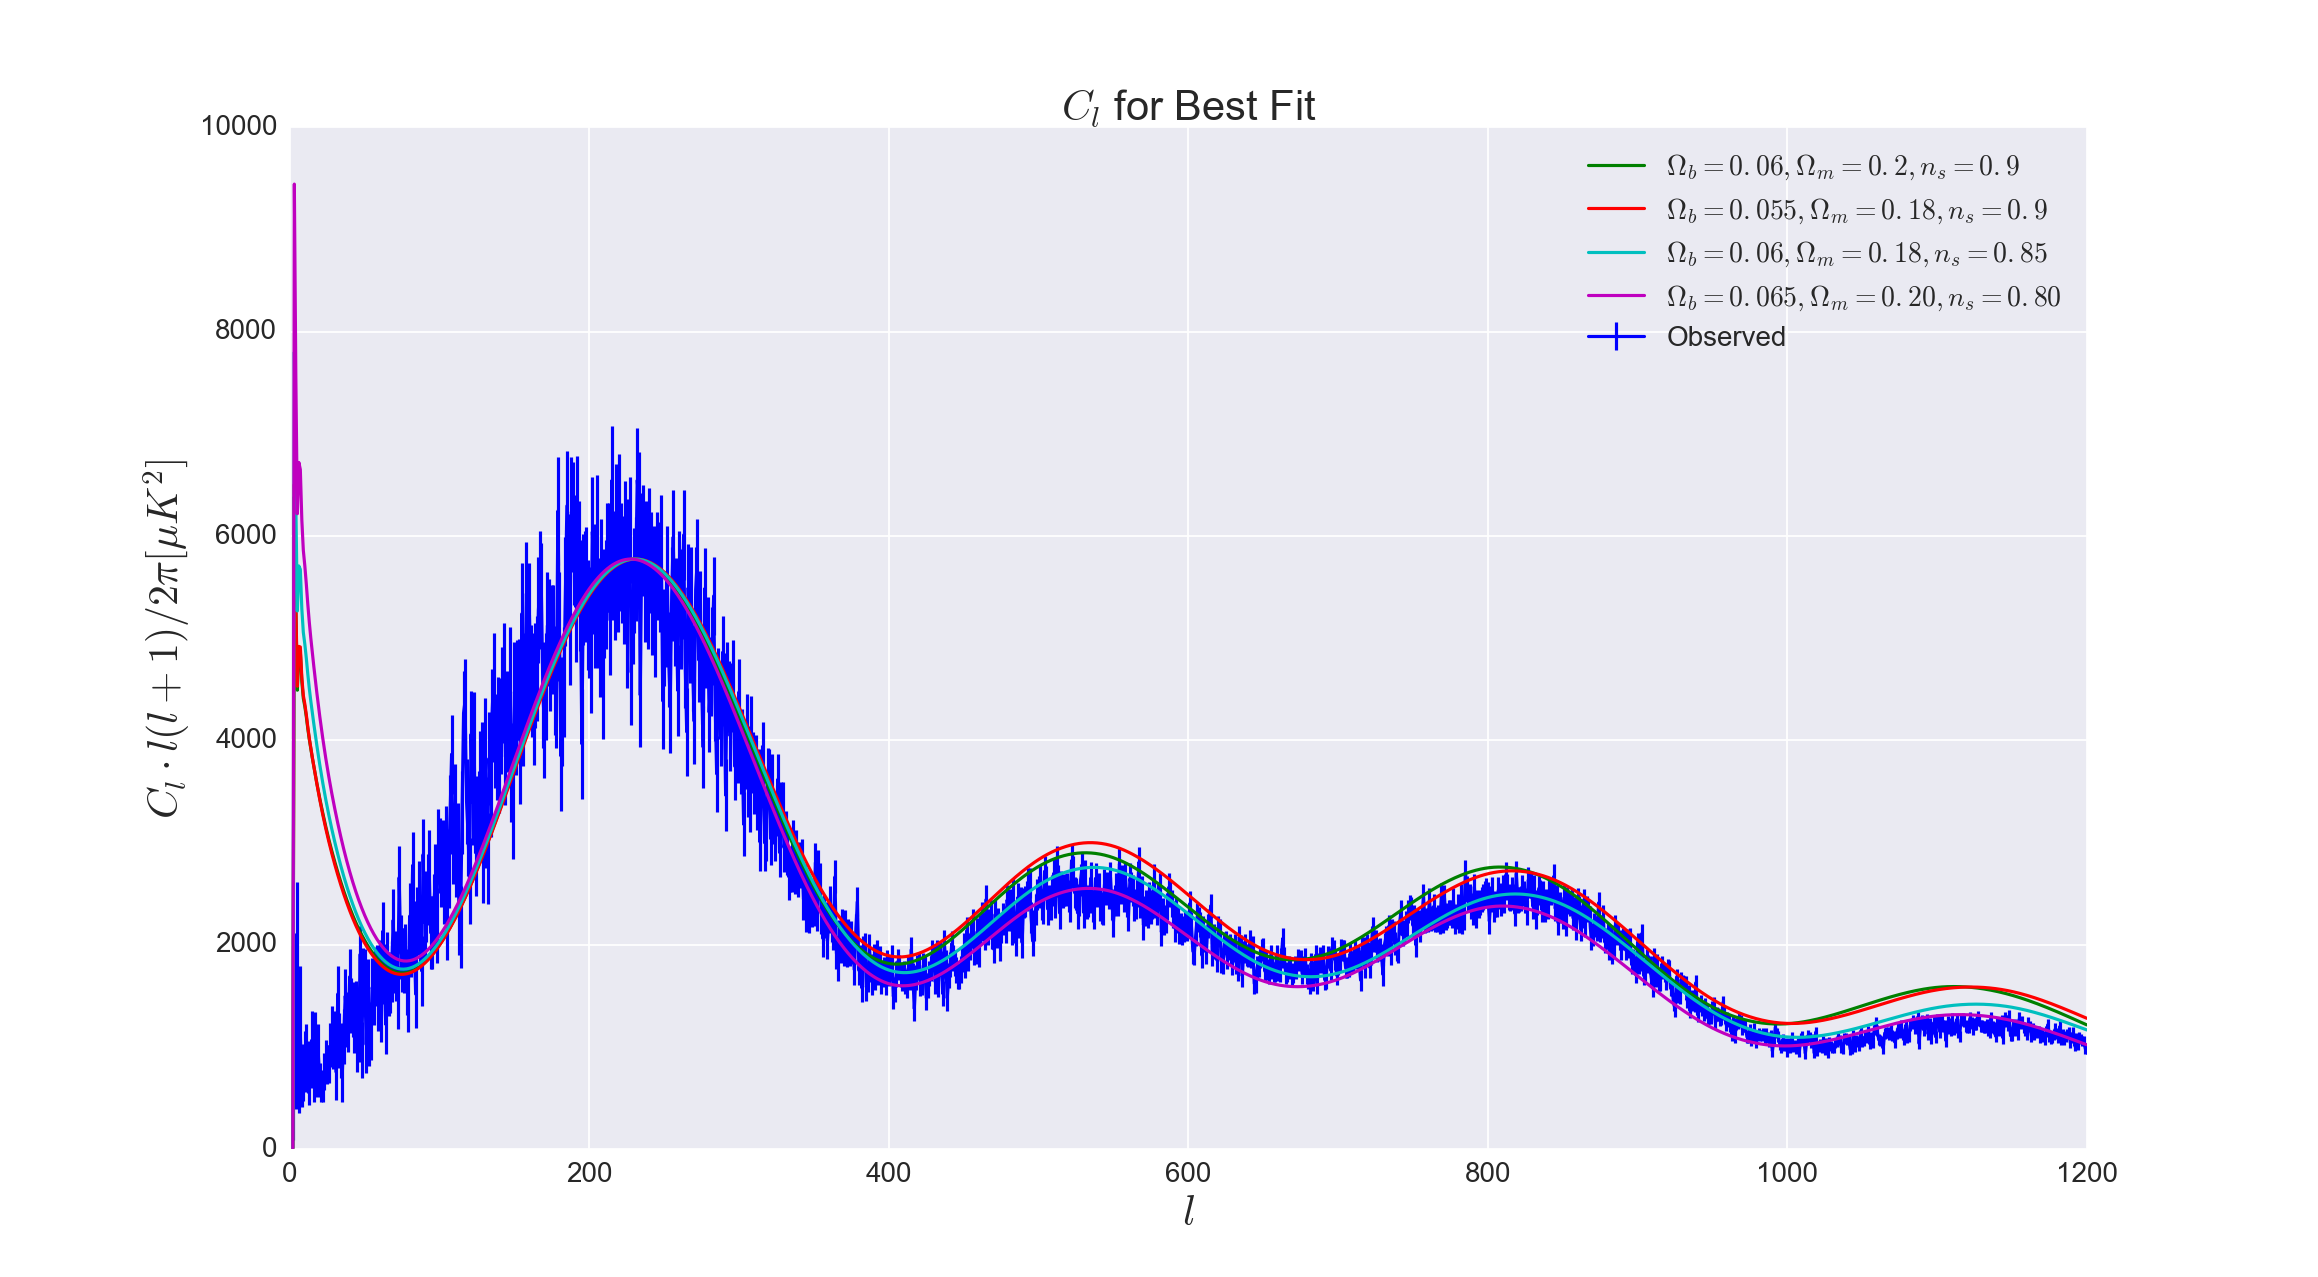
\includegraphics[scale=0.25]{Cl_bf.png}
\caption{The power spectrum $C_l l(l+1)/2\pi$ in $\mu K^2$. I chose the purple as the best fit, but a better fit would be somewhere between the light blue and purple.}\label{fig:Cl_bf}
\end{figure}

\section{Conclusion}

We have finally managed to take the theory and make a power spectrum with can be compared with real observations,fig. \ref{fig:Cl_bf}! We were so able to find estimations of the cosmological parameters based on the observations, tab. \ref{tab:parameters}. The estimations fitted the observations quite well, except for at low $l$s. There are some problems here which I did not have the time to debug.

Even though the best fit curve correlated well with the data, it was not the same parameters found by the Planck team. This is most likely due to the fact that polarization is ignored in this analysis\footnote{And that the Planck team is way better at parameter estimation than me...}!

But all in all the result was very satisfying, and the way there very educational!


\subsection{Notes on my own work}
My code runs mostly without problems, but there are two things that could have been done better. The first is the speed. To integrate the differential equations for $100$ $k$s and calculate the power spectrum, the code takes about $15-20$ min. This is shorter than for some students, but also much longer than other. I've used many hours, but have yet to find the reason. It is not a big problem, but makes debugging a hassle. The second problem is the sharp increase in the power spectrum at $l\lesssim 70$. I've compared my code to other student's code, who does not have this problem, without being able to find the reason. I think the problem is to be found in the code of earlier milestones, but I have yet to find it, and with the long(ish) run time, this process of debugging take too long.

The code for all the milestone can be found at \url{https://github.com/dulte/AST5220}

\begin{thebibliography}{9}

\bibitem{callin}
  Callin, Peter,
  \textit{How to calculate the CMB spectrum},
  astro-ph/0606683
  2006.

\end{thebibliography}


\end{document}

